\documentclass[letterpaper,12pt,notitle]{memphisthesis}                     % the template uses 12pt Arial, I use 12pt Times New Roman
\usepackage[lmargin=1in,rmargin=1in,tmargin=1in,bmargin=1in]{geometry}  % left margin of the original template has been modified
\usepackage[section]{placeins}  % noted by Yu Geng: use this opition to enforce figures to stay in the current section
% \usepackage[demo]{graphicx}   % noted by Yu Geng: use this to speed up compilation, comment it before final render

\usepackage{natbib}         % bibliography showing “and” instead of “&”
\newcommand\harvardand{\&}  % required by the University of Memphis Thesis Style Guide

%\usepackage{chngcntr}
%\counterwithout{figure}{chapter}  % consecutive numbering of tables and figures throughout the document
%\counterwithout{table}{chapter}   % required by the University of Memphis Thesis Style Guide

\usepackage{titlesec}               % move section and subsection titles to the left side a little bit
\titlelabel{\llap{\thetitle\quad}}  % suggested by the Graduation Analyst
\renewcommand\thesection{}     % remove numbering before any section, subsection... names
\renewcommand\thesubsection{}  % required by the University of Memphis Thesis Style Guide

%\usepackage[finalnew]{trackchanges}  % Accept all edits.
\usepackage[inline]{trackchanges}  % Display edits inline.
\addeditor{HC}  % arranged in alphabetical order
\addeditor{EC}  % arranged in alphabetical order


% noted by Yu Geng: usage of [] after \subfigure
% without using [], numbering of subfigures (a) and (b) will not show up
% contents in the [] can be just left as blank
% EXAMPLE
% \begin{figure}
%     \subfigure[]{...}
%     \subfigure[]{...}
%     ...
% \end{figure}

% If you want the fonts to be Times New Roman uncomment the following line 
\usepackage{times}

%If you want the fonts to be Times New Roman, comment out the following 3 lines
% \usepackage[T1]{fontenc}
% \usepackage[scaled]{uarial}
% \renewcommand*\familydefault{\sfdefault}

\usepackage{amsmath}
\usepackage{textcomp}
\usepackage{booktabs}
\usepackage{setspace}
\usepackage{graphicx}
\usepackage{subfigure}
\usepackage[justification=raggedright,
singlelinecheck=false]{caption}
\usepackage{indentfirst}
\usepackage[splitrule]{footmisc}
\usepackage{url}

\setlength{\footnotemargin}{0.5in}
\setlength{\footskip}{0.5in} 

\makeatletter
\let\splitfootnoterule=\pagefootnoterule
\makeatother

\setcounter{tocdepth}{3}
\raggedright

\makeatletter
\let\l@figureOLD \l@figure
\renewcommand{\l@figure}{\vspace{\baselineskip}\l@figureOLD}
\let\l@tableOLD \l@table
\renewcommand{\l@table}{\vspace{\baselineskip}\l@tableOLD}
\makeatother

\setlength{\parindent}{0.5in}

\begin{document}

\pagenumbering{roman}

\begin{titlepage}

\vspace*{.66in}
\begin{center}\uppercase{
New Numerical Mid-Ocean Ridge Models for Interactions between plate-driving and resistant forces 
}\vspace{2em}\\  % \vspace{.34in}\\
by\\
\vspace{2em}  % \vspace{.34in}
Hee Choi
% Interactions between plate-boundary forces and evolving resistance at mid-ocean ridges as the origin of non-uniform seafloor growth

\vspace{1.5in}
A Thesis \\
\vspace{14pt}
Submitted in Partial Fulfillment of the\\ \vspace{14pt}
Requirements for the Degree of\\ \vspace{14pt}
Master of Science
\vspace{0.5in}

Major: Earth Sciences

\vspace{1.66in}
The University of Memphis \\
\vspace{14pt}
May 2019
\end{center}

\end{titlepage} 


\doublespacing
\widowpenalty=10000

\setcounter{page}{2}

%\begin{center}
%	\textbf{ACKNOWLEDGEMENTS}
%\end{center}
%\vspace{-0.15in}
%
%Acknowledments~

\newpage
\begin{center}
	\textbf{ABSTRACT}
\end{center}
\vspace{-0.15in}

\thispagestyle{plain}

Evidence for asymmetric plate growth, variable crustal thickness, and non-uniform spreading rates is ubiquitous on the seafloor. However, conventional numerical modeling approaches are often incapable of explaining the non-uniform growth of oceanic lithosphere. Noting that plate-boundary forces can dynamically determine plate speed by finding a balance against the resistance to extension at ridge axes and at lithosphere-asthenosphere boundary, I introduce plate-boundary forces instead of kinematics to drive plate motions in numerical models for mid-ocean ridges. I construct such models using FLAC, an open-source finite element code for geodynamic simulations. My mid-ocean ridge models tested three different boundary conditions: Prescribed velocities, zero boundary force, %$(\boldsymbol{F_{res}})_x$ equals to zero models, 
and constant non-zero boundary force. All three types of boundary conditions can produce faulting styles consistent with the previous studies but mean plate speeds respond differently to different boundary condition types. Mean plate speed is almost constant in the kinematic and zero boundary force models. The constant non-zero force boundary conditions make plates move at 1.8 cm/yr of mean speed, but plate speed changes over time by more than 1 cm/yr. These model results suggest that even if far-field plate-driving forces are nearly constant, non-uniform seafloor growth can result. However, further investigation is necessary for reducing numerical noise and extracting mean plate speed with greater confidence.

\newpage

\begin{singlespace}
	\tableofcontents
\end{singlespace}

\newpage

\addcontentsline{toc}{chapter}{List of Figures}

\addtocontents{lof}{\vspace*{-\baselineskip}}

\begin{singlespace}
	\listoffigures
\end{singlespace}

\newpage

\pagenumbering{arabic}

\chapter{Introduction}
\setcounter{section}{0}
\setcounter{subsection}{0}

Mid-ocean ridge systems have been extensively studied because of their unique geological and geophysical characteristics as well as their importance in global plate tectonics. Being the longest mountain belt on the Earth, mid-ocean ridges have a total length of 80,000 km and cover over 23 percent of the Earth’s surface \citep{Peltier1989}. Stripe patterns of magnetic anomalies parallel to the mid-ocean ridge are critical evidence for seafloor spreading and the birth of plate tectonics \citep{Hess1964}.

The mid-ocean ridge is the place where new oceanic crust and lithosphere are generated by partial melting of the upper mantle \citep{Cann1968}. Magma rising from the upper mantle extrudes onto the ocean floor and bonds to the edges of separating plates \citep{Chen1992}. The oceanic plates start to thin and thicken by the underplating of the new lithosphere from the upper mantle and the accumulation of overlying sediment layers. As it moves away from the ridge, the lithosphere gets cooler and denser.

Previous studies for mid-ocean ridges have improved our understanding of how rheological and thermal structures affect faulting at a mid-ocean ridge system.
%\citet{Lavier2002} suggested that the hydrothermal circulation determine the style of faulting on both half grabens and large-offset low-angle normal fault.\note[EC]{Lavier2002 seems out of context. Maybe later when you discuss large-offset normal fault?} 
\citet{Cannat1993} suggested the discontinuous magmatic crust model the emplacement of mantle rocks characterize the near-axis region of slow-spreading ridge. Observed axial serpentinized peridotites support the idea of uplifted mantle material. Using flexural fault models, \citet{Escartin1997} investigated what affects the normal fault spacing at slow-spreading ridges. Lowering the friction coefficient caused by sepertinization affects more than lithospheric thickness variations caused by temperature variation. With abundant serpentinites, faults are widely spaced and have large heaves at the ridge segment ends, while faults are small and closely spaced at segment centers when serpentinites are scarce. \citet{Singh2006} provided the first seismic reflection image of a subsurface near-magma chamber at slow-spreading ridges and a series of inward-dipping faults cutting through the volcanic edifice, suggesting a continuous interplay between magmatic and tectonic processes. \citet{Reston2011} claimed that both a large-offset normal fault and a series of comparatively small fault blocks are likely to originate through a rolling hinge mechanism, caused by the flexure of the footwall during unloading. When the fault locks up at an adequately high angle, a new fault propagates upward from the active root zone. Repeating these processes produces a series of small rafting fault blocks.

Numerical models including the relationship between dike opening rate and plate separation have also significantly contributed to the knowledge of faulting at mid-ocean ridges and diversity of seafloor morphologies. %\note[EC]{I think Chen and Morgan, Behn and Ito, Ito and Behn, Olive all should be a part of this paragraph. In the previous one, you can combine Reston, Singh, Cannat, J. Escartin, P. Canales etc.}
\citet{Chen1990} coupled the thermal and rheological structures in a model of lithospheric stretching to consider the controls on axial relief at mid-ocean ridges. The spreading rate dependence of axial valley morphology is well predicted by including a weak lower crust with power-law rheology. \citet{Buck1998} developed a simple way to parameterize the complex process of magmatic accretion at a spreading center. This numerical model assumes steady accretion of crust at the spreading center. \citet{Buck2005} and \citet{Tucholke2008} showed that differences in magmatic input to dikes produce the different modes of faulting at mid-ocean ridges. When magmatic accretion accommodates 30-50\% of spreading, the model generates detachment faults while the model shows alternating faulting mode when most of the spreading is accommodated by magmatic accretion. 
\citet{Behn2008} explored several factors including lithospheric thickness and rheological structure that can control fault growth. The dominant factor they found was the ratio of magmatic accretion rate to total plate spreading rate. When this ratio approaches 0.5, the model produces larger and widely spaced faults.
\citet{Ito2008} introduced the rise-sink ratio, a parameter that controls the transition between axial topographic highs and median valleys. Models predict tall axial highs when the rise-sink ratio is significantly larger than 1 and axial valleys when the ratio is smaller than 1. The topography of the Galapagos spreading center and the Southeast Indian ridge are well-explained by this relationship.
\citet{Olive2015} looked at the pattern of faulting by varying the period of magmatic fluctuation. Increasing the period of fluctuating magma supply in the model generates long-wavelength topography with large-offset faults.
\citet{Tian2017} used three-dimensional models to quantify the effects of axially variable diking rates on faulting at slow spreading ridge segments and newly identified transitional mode. Varying the amount of magma supply along the spreading axis results in two different faulting modes in one model, which is a transitional mode.

\begin{figure}[!htb]
	\centering
	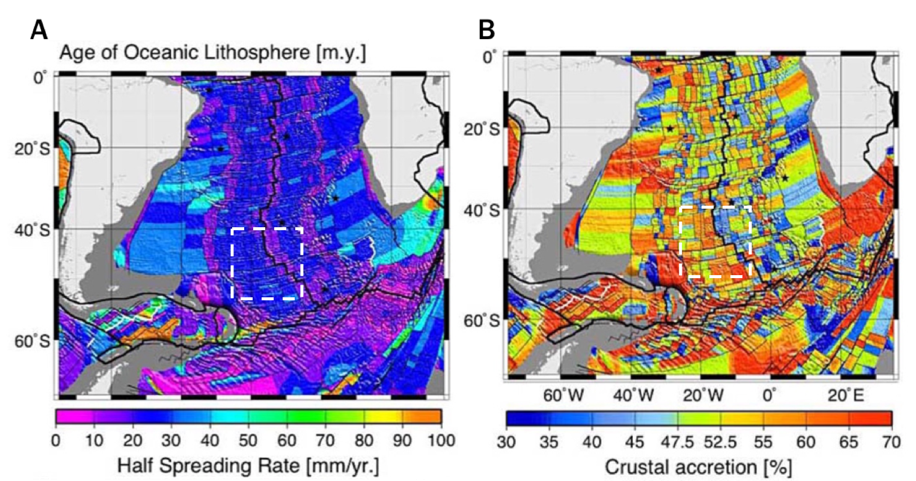
\includegraphics[width=0.9\linewidth,trim=4 4 4 4,clip]{./figs/hsr_muller.png}
	\caption{\textbf{A.} Seafloor half-spreading rates. \textbf{B.} Crustal accretion asymmetries in the South Atlantic, Scotia Sea, and northern Weddell Sea. Dashed boxes in A and B mark the region clearly showing asymmetric features. Modified from \citet{Muller2008}}
	\label{fig:hsr_muller}
\end{figure}

These previous numerical modeling studies of mid-ocean ridge have assumed the accretion of oceanic lithosphere at spreading centers symmetrically and at a constant rate, but this assumption is not consistent with various observations \citep{Castelino2016, Flament2014, Martinez2006, Muller1998, Muller2008, Fedotova2017}. \citet{Castelino2016} explained anomalous bathymetry of the Mozambique basin and Riiser Larsen sea with the presence of thicker-than-usual oceanic crust older than 100 Ma. \citet{Flament2014} suggested that viscous lower mantle flow may produce the topographic asymmetry of the South Atlantic. \citet{Martinez2006} identified non-corresponding trends in crustal thickness and spreading rate along the back-arc Eastern Lau Spreading Center. \citet{Muller2008} published global models for seafloor ages, spreading rates, and spreading asymmetry of ocean crust. If the two plates grew symmetrically at every divergent boundary, the spreading rates of the two plates would be the same, and therefore relative proportions of crustal accretion on conjugate ridge flanks would be 50 \% everywhere. However, \citet{Muller2008} models clearly exhibit asymmetries in spreading rates and crustal accretion. For instance, in a South Atlantic region enclosed in white dashed boxes in Fig.~\ref{fig:hsr_muller}A, most of the South American plate shows a half-spreading rate of about 2-3 cm/yr while the youngest ocean basin on the African plate exhibits a lower spreading rate of 1-2 cm/yr. Correspondingly, the crustal accretion asymmetry ratio is 50-60 \% on the South American plate while lower than 50 \% on the African plate. Most importantly, asymmetric plate growth is not specific to a particular region: It is a worldwide feature~\citep{Muller2008}.
%
\begin{figure}[!htb]
	\centering
	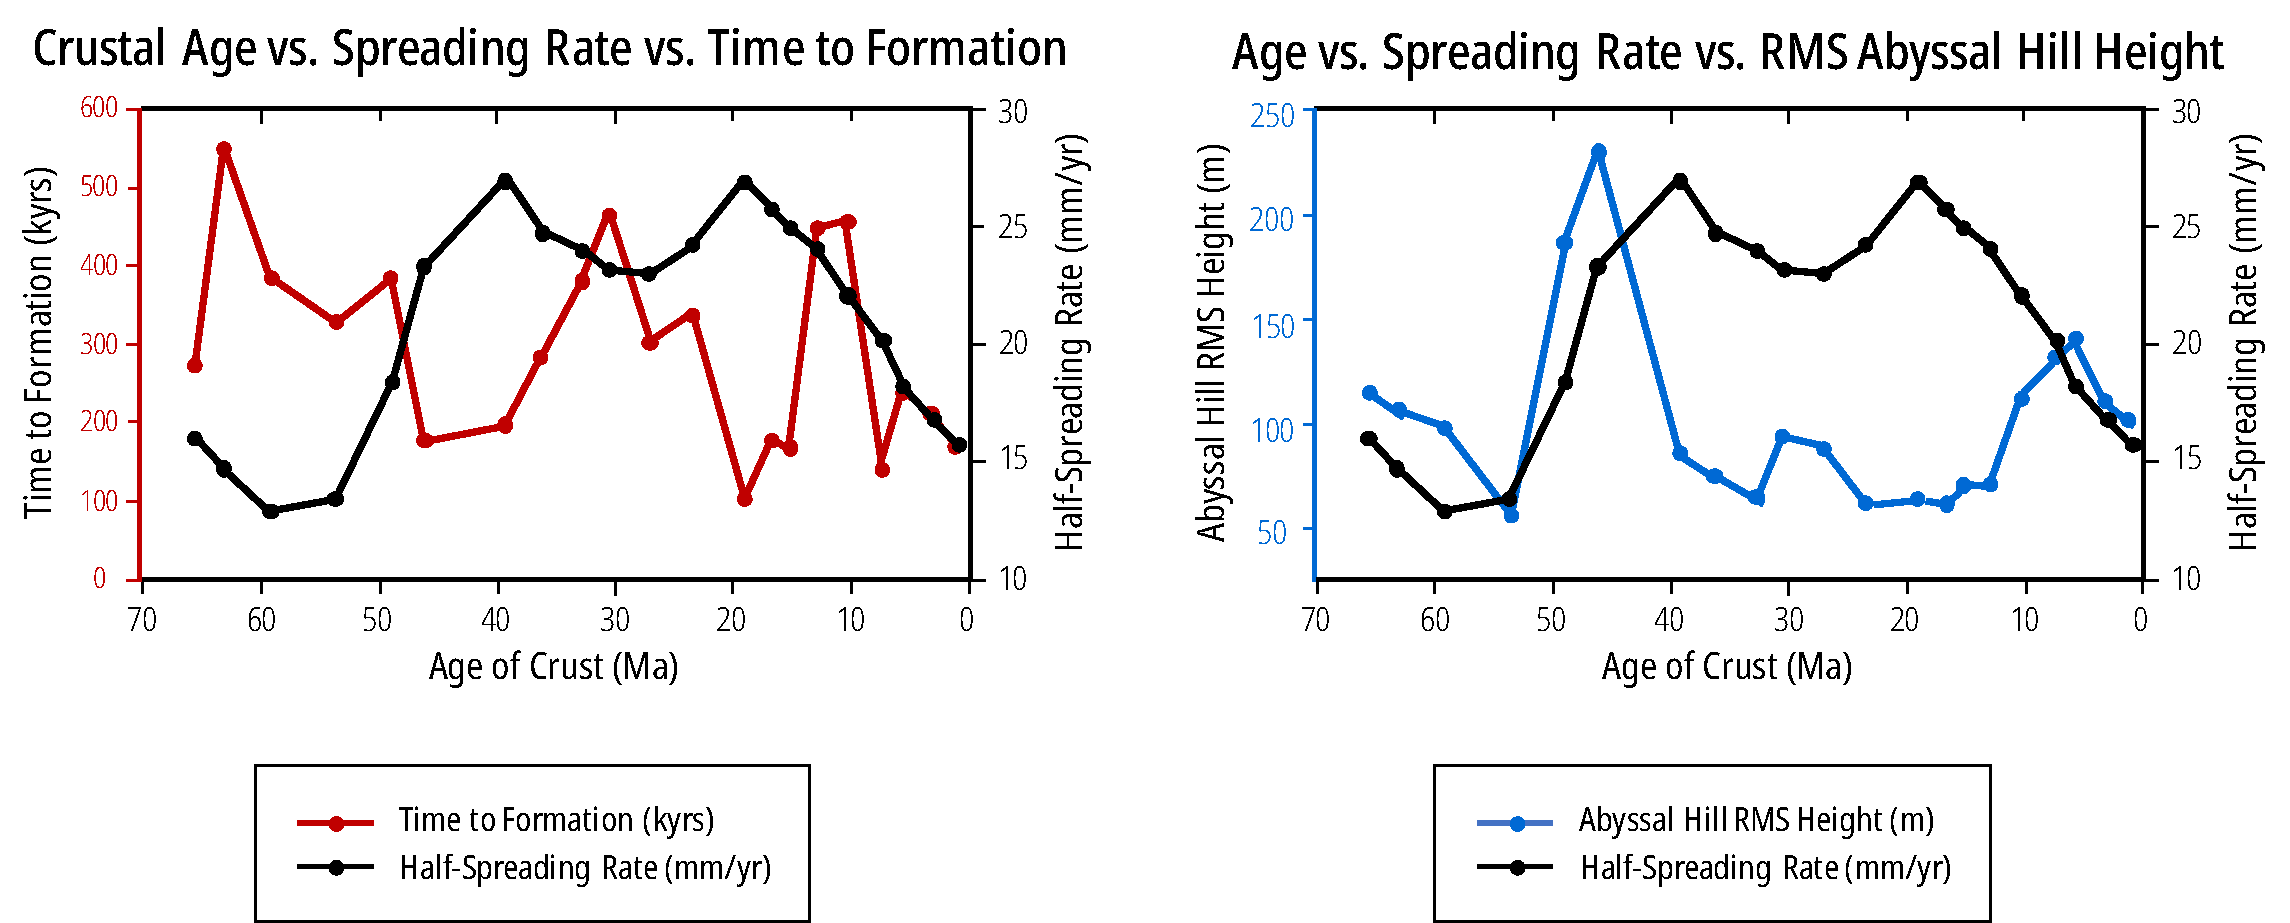
\includegraphics[width=0.99\linewidth]{./figs/hsrgraph1.pdf}
	\caption{Non-uniform half-spreading rate, abyssal height and time to form abyssal hill data from CREST expedition in mid-Atlantinc Ridge. Digitized from \citet{Fedotova2017}}
	\label{fig:hsr_fedotova}
\end{figure}

The rate of plate growth is not only asymmetric across divergent boundaries but also variable in time. Evidence can be found in the global spreading rates compiled by~\citet{Muller2008} as well as in regional surveys like CREST (Crustal Reflectivity Experiment Southern Transect)~\citep{Fedotova2017}. Data collected in the CREST expedition include half-spreading rates, times taken to form abyssal hills and abyssal hill heights. If plates grew at a constant rate, spreading rates and required times to form abyssal hills would be constant and abyssal hill heights would be plotted as a sinusoidal curve with regular amplitude and frequency by assuming uniform plate spreading. However, the CREST data show significant variations in these observables over time (Figure \ref{fig:hsr_fedotova}). For instance, the spreading rate varies by 15 mm/yr over the period of about 70 Myrs. Time taken to form abyssal hill varies by 450 Kyrs throughout about 70 Myrs. These observations indicate non-uniform plate growth behavior on the seafloor.
%
Additional evidence for both time-varying and asymmetric seafloor growth comes from SCARF(Student-led Cruise Along a Ridge Flow Line) cruise to the northern Mid Atlantic Ridge~\citep{Shinevar2018} (Fig.~\ref{fig:scarf}A). Calculated spreading rates from the collected magnetic data (Fig.~\ref{fig:scarf}B) along a $\sim$700 km-long transect across the ridge axis show twice higher half-spreading rates compared to the near-axis region. Half-spreading rate would remain constant if seafloor grew uniformly. Besides, the half-spreading rate is 10 mm/yr within 100 km to the west from the ridge axis but is 15 mm/yr over the same distance to the east of the axis. The spreading and plate growth at this ridge has been asymmetric. 
%
\begin{figure}[!htb]
	\centering
	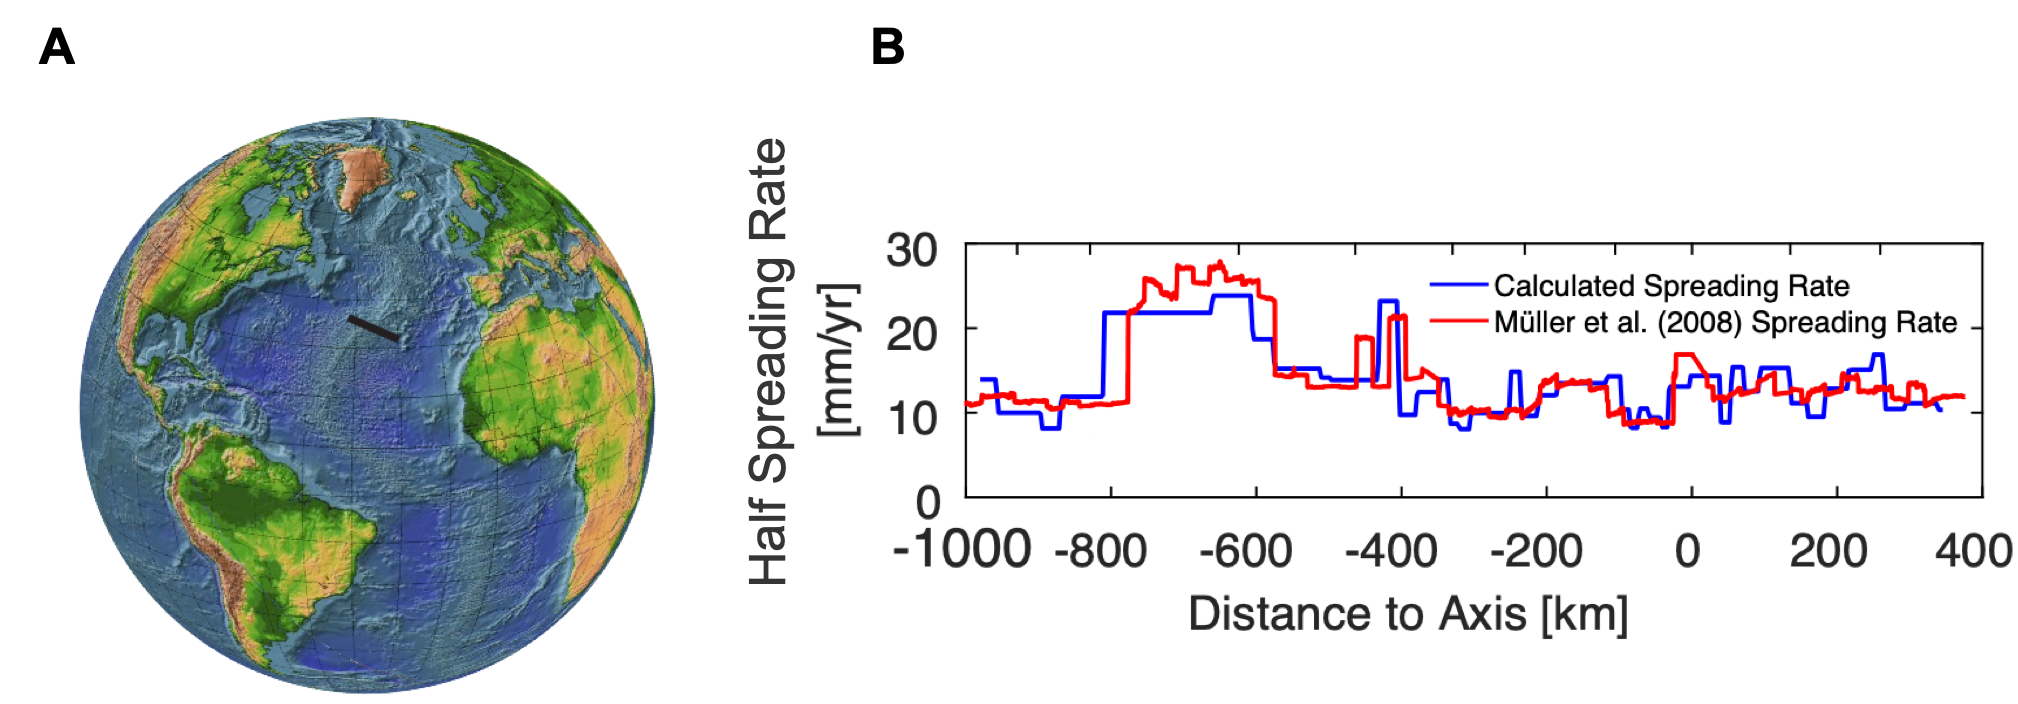
\includegraphics[width=0.85\linewidth,trim=4 4 2 12,clip]{./figs/scarf.png}
	\caption{\textbf{A.} Location of SCARF cruise. Black line is the cruise trackline. \textbf{B.} Calculated half-spreading rate from measured magnetic data. From \citet{Shinevar2018}.}
	\label{fig:scarf}
\end{figure}


Continental rifts, another type of divergent plate boundary, has recently been shown to form slowly during the incipient stage and accelerate later \citep{Brune2016}. Kinematic modeling based on plate motion inversion data from the major passive margins of North Atlantic, North America – Greenland, Australia – Antarctica, and the South China sea, \citet{Brune2016} identified several rapid changes in absolute plate motion from the extension records in the major passive margins around the world, which have not been explained previously. They explained the multi-phase rifting as a result of the interaction between the rift-intrinsic strength and forces pulling the plates apart. At the initial stage of rifting, the lithosphere is still thick and strong, and thus, high strength slows rifting (Figure \ref{fig:brune}A). When the lithosphere gets significantly thinned and weakened, low strength enables fast rifting (Figure \ref{fig:brune}B).
%
\begin{figure}[!htb]
	\centering
	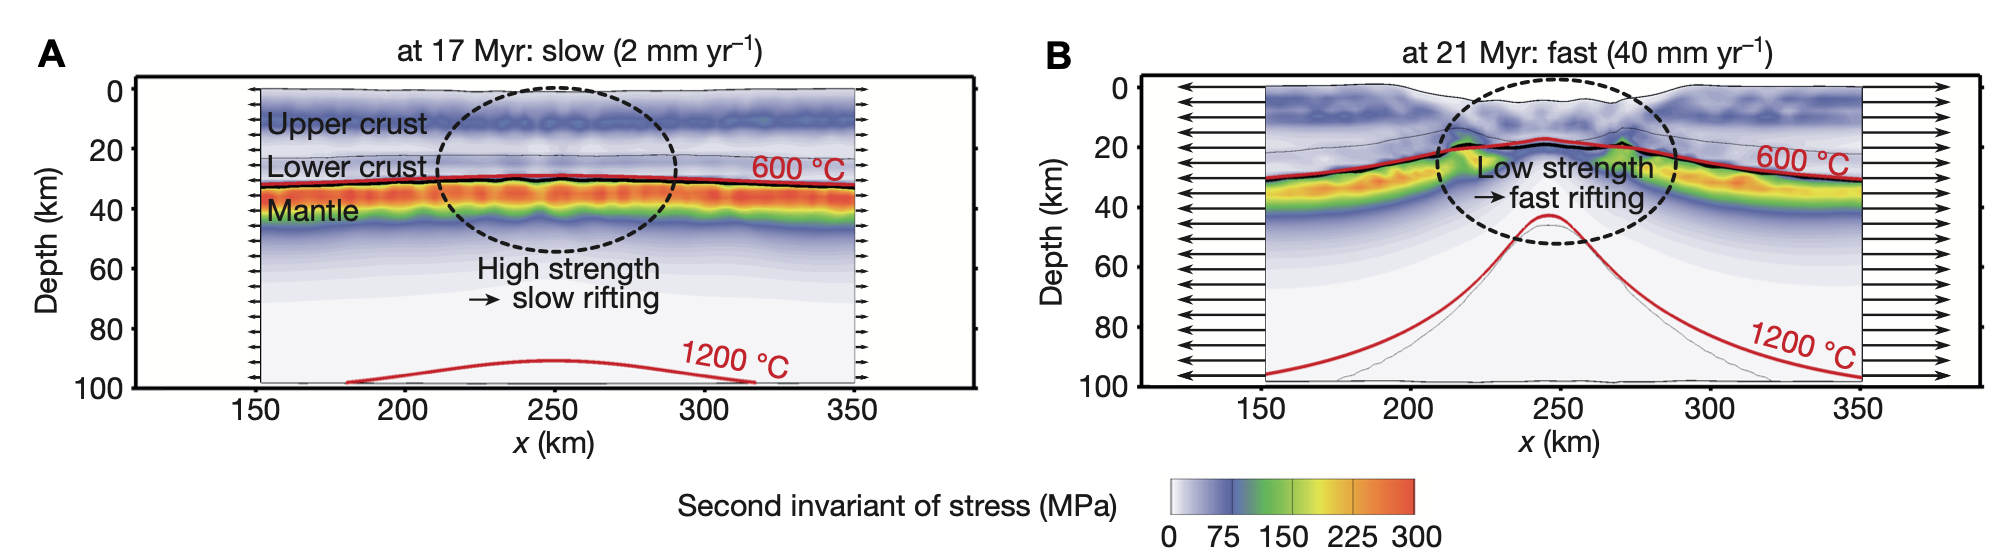
\includegraphics[width=0.99\linewidth,trim=4 4 4 4,clip]{./figs/brune.png}
	\caption{Strength evolution in numerical models for continental rifting with constant force boundary conditions. \textbf{A.} Distribution of the second invariant of stress at 17Myr when the lithosphere is still thick and strong and thus the extension rate is low, 2mm/yr. Arrows indicate extension velocity. \textbf{B.} After 21Myr when the lithosphere gets significantly thinned and weakened, letting the extension rate increase to 40 mm/yr. From \citet{Brune2016}}
	\label{fig:brune}
\end{figure}

Prompted by the non-uniform plate growth at mid-ocean ridges and potential interactions between the far-field forces and mid-ocean ridge processes, I develop new numerical models that can be useful for investigating how interactions between plate driving forces and internal forces would affect spreading rates of oceanic plates. My models will be built upon existing mid-ocean ridge modeling techniques for simulating diking and faulting at spreading centers because magmatism and faulting play a vital role in determining characteristics of oceanic lithosphere that can be compared to observations. My new contribution is to replace conventional kinematic boundary conditions with traction boundary conditions in a popular open-source code for geodynamic modeling and investigate the effects of the traction boundary conditions on lithospheric growth. In the next sections, I describe the modeling method used in my study, show and discuss model results and challenges involved in interpreting them. The main findings are summarized at the end.

\chapter{Modeling Method}

\section{Background: Magmatism, faulting and seafloor morphology}
Magmatism at the spreading center of mid-ocean ridges plays an essential role in determining faulting styles that in turn control the axial and seafloor morphology. At fast-spreading ridges, copious magma rises and forms axial high (Figure \ref{fig:ridgebathymetry}A). With abundant magma, diking can occur frequently accommodating a significant portion of plate separation. For this reason, faults forming near axial highs have only small (i.e., 100s m) offsets (Figure \ref{fig:ridgebathymetry}A). Density variations are significant across fast-spreading ridges since the axial lithosphere is very thin, hot, and underlain by the partially molten crust. Axial highs might originate from molten magma rising to the level of local isostatic equilibrium at the plate spreading axis and then subsiding as it cools down. In contrast, faults forming at slow-spreading centers show greater offset, and axial valleys form at the spreading center (Figure \ref{fig:ridgebathymetry}B). Less abundant magma compared to fast-spreading ridges means less frequent diking and tectonic stretching accommodates a significant portion of plate separation. Faults at slow-spreading ridges develop offset up to 1-2 km. Abyssal hills produced at slow-spreading ridges are composed of faults dipping towards the axis while about half of the faults near fast-spreading centers dip toward the axis and the other half dip away from the ridge axis.

\begin{figure}[!htb]
	\centering
	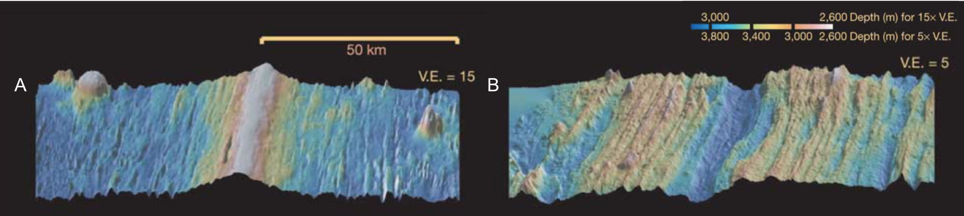
\includegraphics[width=0.99\linewidth]{./figs/bathy_buck.png}
	\caption{Shaded relief images of bathymetry at slow and fast ridges. \textbf{A.} The East Pacific Rise along 9$^\circ$37$'$N latitude \textbf{B.} The Southeast Indian Ridge along the 115$^\circ$E segment. Modified from \citet{Buck2005}.}
	\label{fig:ridgebathymetry}
\end{figure}

Assuming a constant magma injection rate at the dike zone, \citet{Buck1998} simplified the complex diking process. They treated the intrusion of a dike of low viscosity magma by specifying the stress on a vertical interface placed at the center of the crust layer. Normal stress is set equal to the lithostatic pressure in the crust layer, and shear stress is set to zero on the interface.
This approach allowed the lateral position of a modeled dike to explain the contrasting faulting styles at slow- and fast-spreading ridges.

\begin{figure}[!htb]
    \centering
    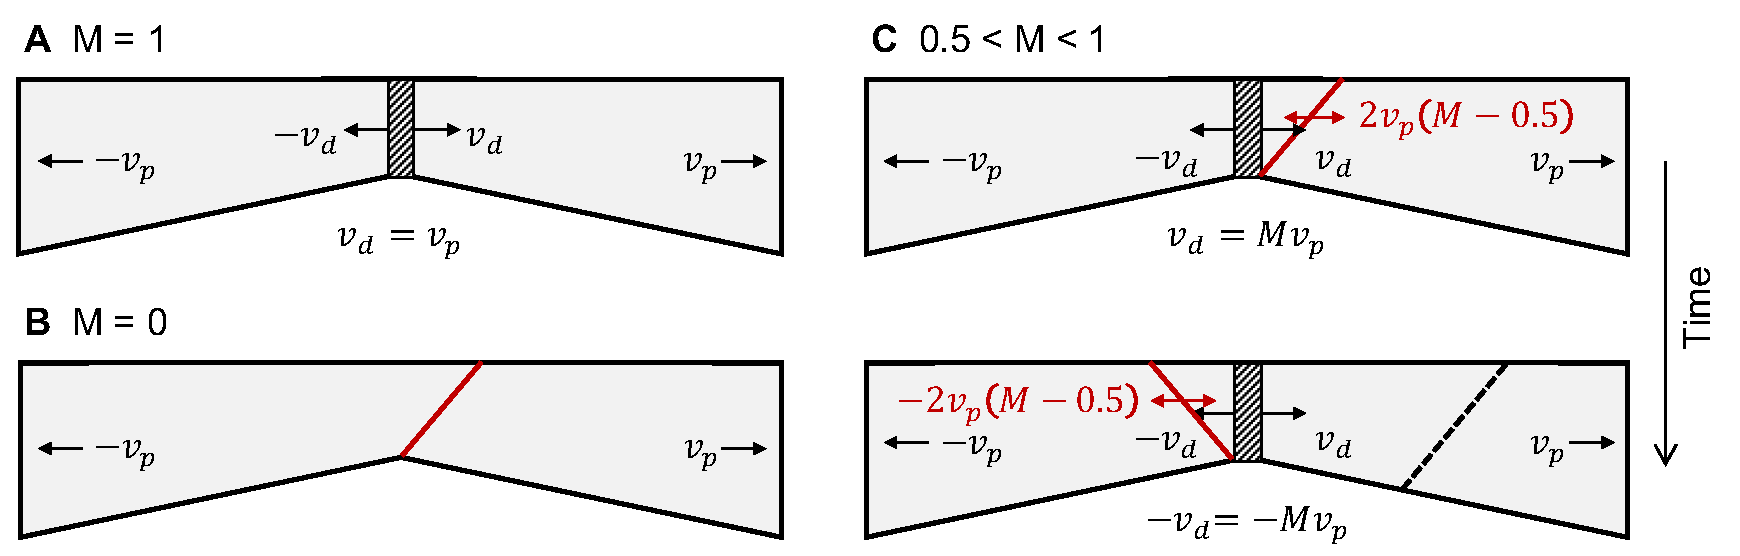
\includegraphics[width=0.99\linewidth]{./figs/mfactor.pdf}
    \caption{Cartoon showing how M factor determine plate separation mechanism. \textbf{A.} M $=$ 0, all extension is taken up by fault. No diking occurs. \textbf{B.} M $=$ 1, dike accommodates all extensions. Dike opening rate and plate separation rate are same. \textbf{C.} 0.5 $<$ M $<$ 1, more than half of plate separation is accommodated by dike and hence faults migrate off axis. It shows how the hanging-wall block of a fault may migrate during ridge stretching.}
    \label{fig:mcartoon}
\end{figure}

\section{M factor parametrizing plate separation by diking}
\citet{Buck2005} introduced the ratio of dike opening rate to total plate spreading rate as a parameter for numerical mid-ocean ridge models. This ratio is denoted as M, and when given as a parameter for a model, it determines the rate of diking-accommodated plate separation as M times total spreading rate. When M $=$ 0, dikes account for none of the plate spreadings (Fig.~\ref{fig:mcartoon}A); and dikes accommodate all the plate separations when M $=$ 1 (Fig.~\ref{fig:mcartoon}B). M $<$ 1 corresponds to the case where magma supply is insufficient for filling the entire opening created by plate separation and tectonic stretching of the lithosphere should occur. For M = 1, axial lithospheric separation is all taken up by dike widening and no faults or axial valleys develop. For 0.5 $<$ M $<$ 1, faults develop and migrate away from the axis at a rate of $v_d-v_p$, where $v_{p}$ is the half-spreading rate and $v_{d}$ is the dike opening rate defined as $2Mv_{p}$. Thus, $v_{d}-v_{p}$ is equal to $2 v_p (M - 0.5)$ (Fig.~\ref{fig:mcartoon}C). 
%\annote[EC]{2$v_p$ (M $-$ 0.5)}{Explain how this expression is derived.}
%\begin{align}
%v_d - v_p &= 2 M v_p - v_p 
%&( M = \frac{v_d}{2 v_p}) \\
%                &= 2v_p (M - 0.5)
%\end{align}
%(Figure \ref{fig:mcartoon}C). 
The opening by diking is faster than the horizontal component of the fault slip rate when M $>$ 0.5 the fault offset increases, the fault itself is pushed off axis with time. When pushed far away from the axis, the fault locks because the lithosphere around the fault becomes thicker and stronger. As a result, a new fault forms at the spreading center, continuing to accommodate a part of plate separation. 

\subsection{M factor and seafloor morphologies}
Abyssal hills form at mid-ocean ridge spreading centers by magmatism and normal faulting that occurs alternatingly on both sides of the ridge axis. Figure \ref{fig:abyssalhill}A shows the location of Southwest Indian Ridge, a place where abyssal hills are observed and explained as a product of alternating small-offset normal faults. Figure \ref{fig:abyssalhill}B, the bathymetric cross section, displays a symmetric pattern of small-offset faults. Zoom a and zoom b point out the abyssal hills in more detail, offsets of the faults are much smaller than that of detachment fault.
%
\begin{figure}[!htb]
	\centering
	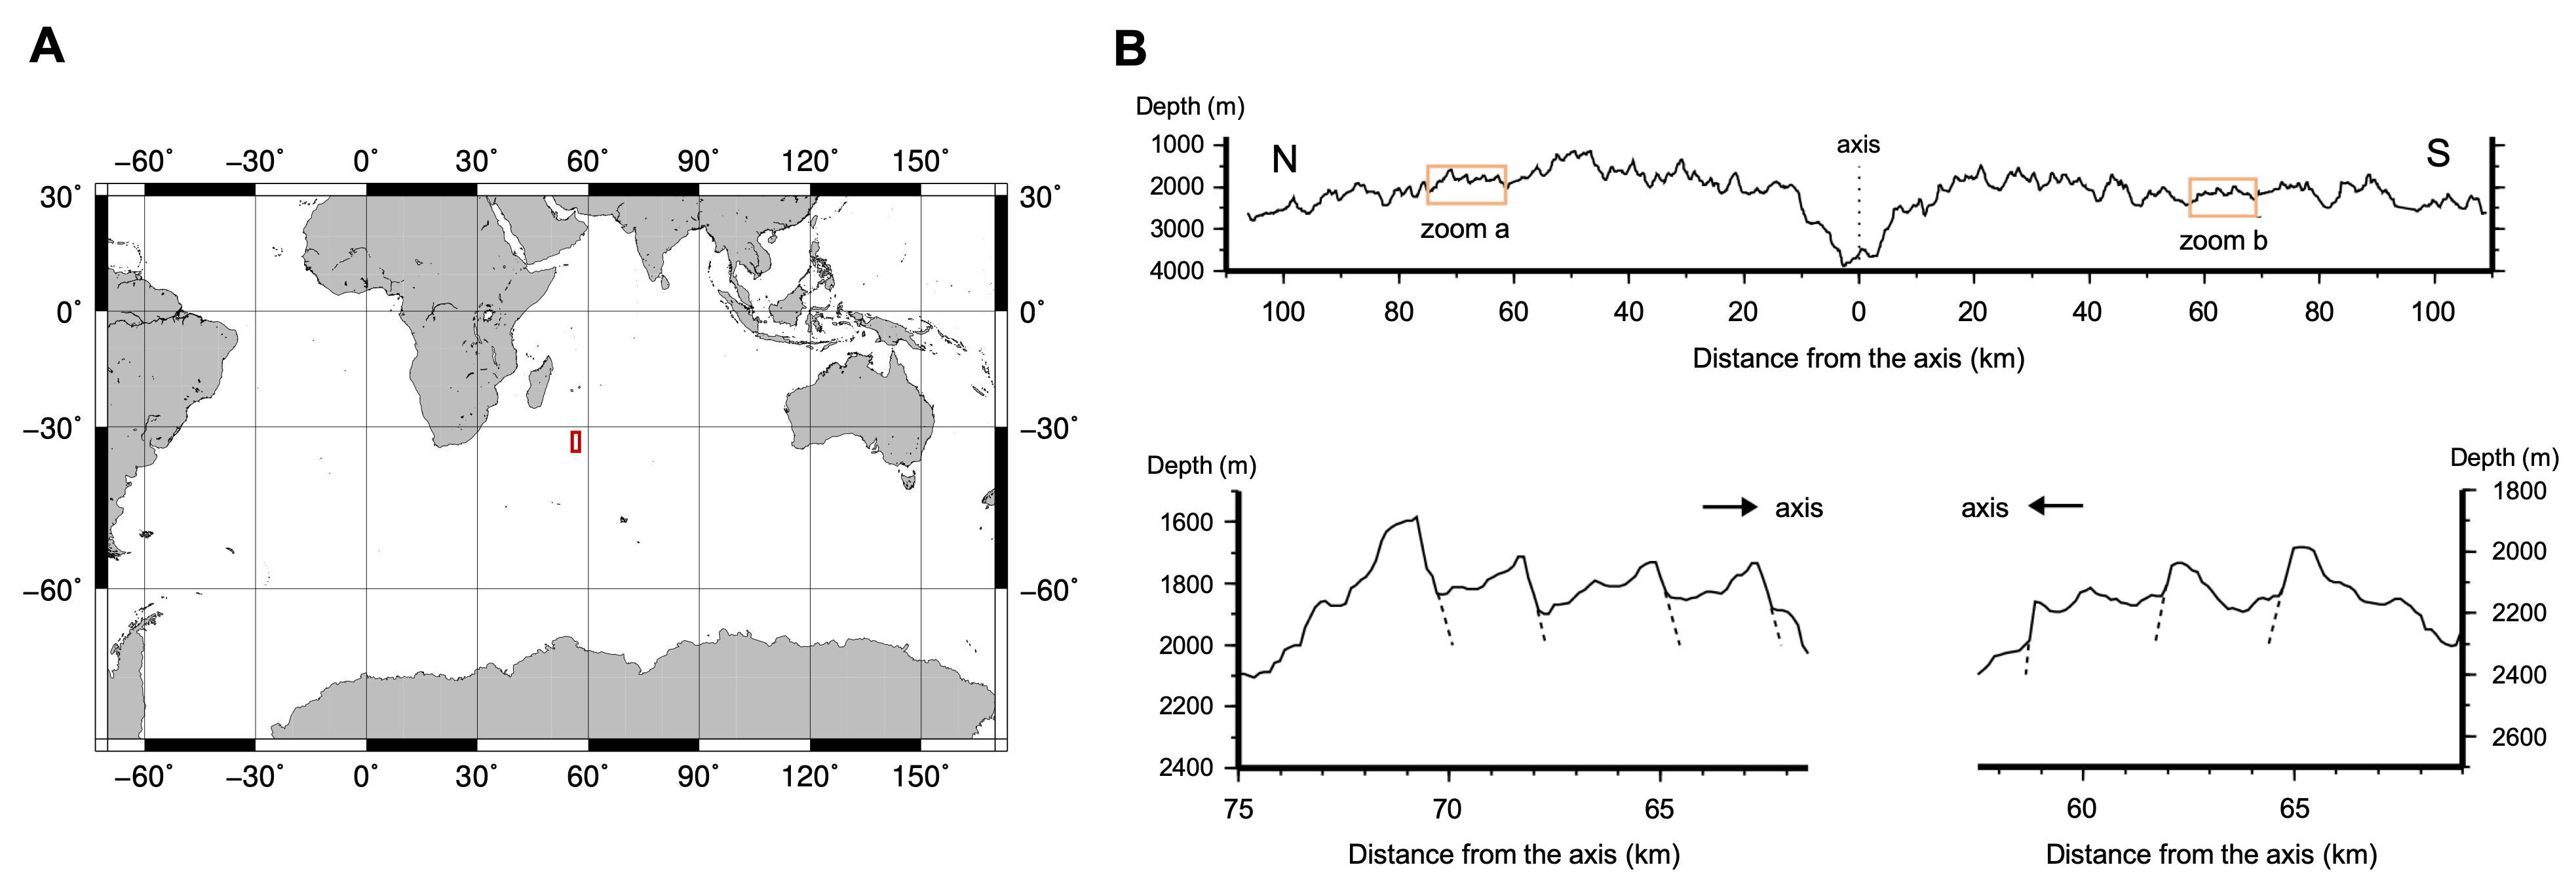
\includegraphics[width=0.95\linewidth,trim=8 8 8 8,clip]{./figs/abyssalhill.png}
	\caption{\textbf{A.} The location of Southwest Indian Ridge (SWIR). Red box points to the area explained in \textbf{B}. \textbf{B.} Bathymetric cross sections along the spreading direction of abyssal hills of SWIR. Zoom a and zoom b clearly point out the small-offset faulting features. Modified from \citet{Mendel2003}}
	\label{fig:abyssalhill}
\end{figure}

Oceanic core complexes(OCCs) have been recognized along slow- and ultraslow- spreading ridges \citep{Tucholke1998}, and are characterized by dome-shaped bathymetric highs interpreted as portions of the lower crust and/or upper mantle exposed by detachment faulting \citep{Tucholke1994}. OCCs form at or near the axis, beneath long-lived ($\sim$1-2 Myr) normal faults which are commonly observed on mid-ocean ridges. Figure \ref{fig:occ} shows an observed detachment fault in multibeam bathymetry data. Detachment near 37 km distance shows $\sim$3000 m depth offset.
%
\begin{figure}[!htb]
	\centering
	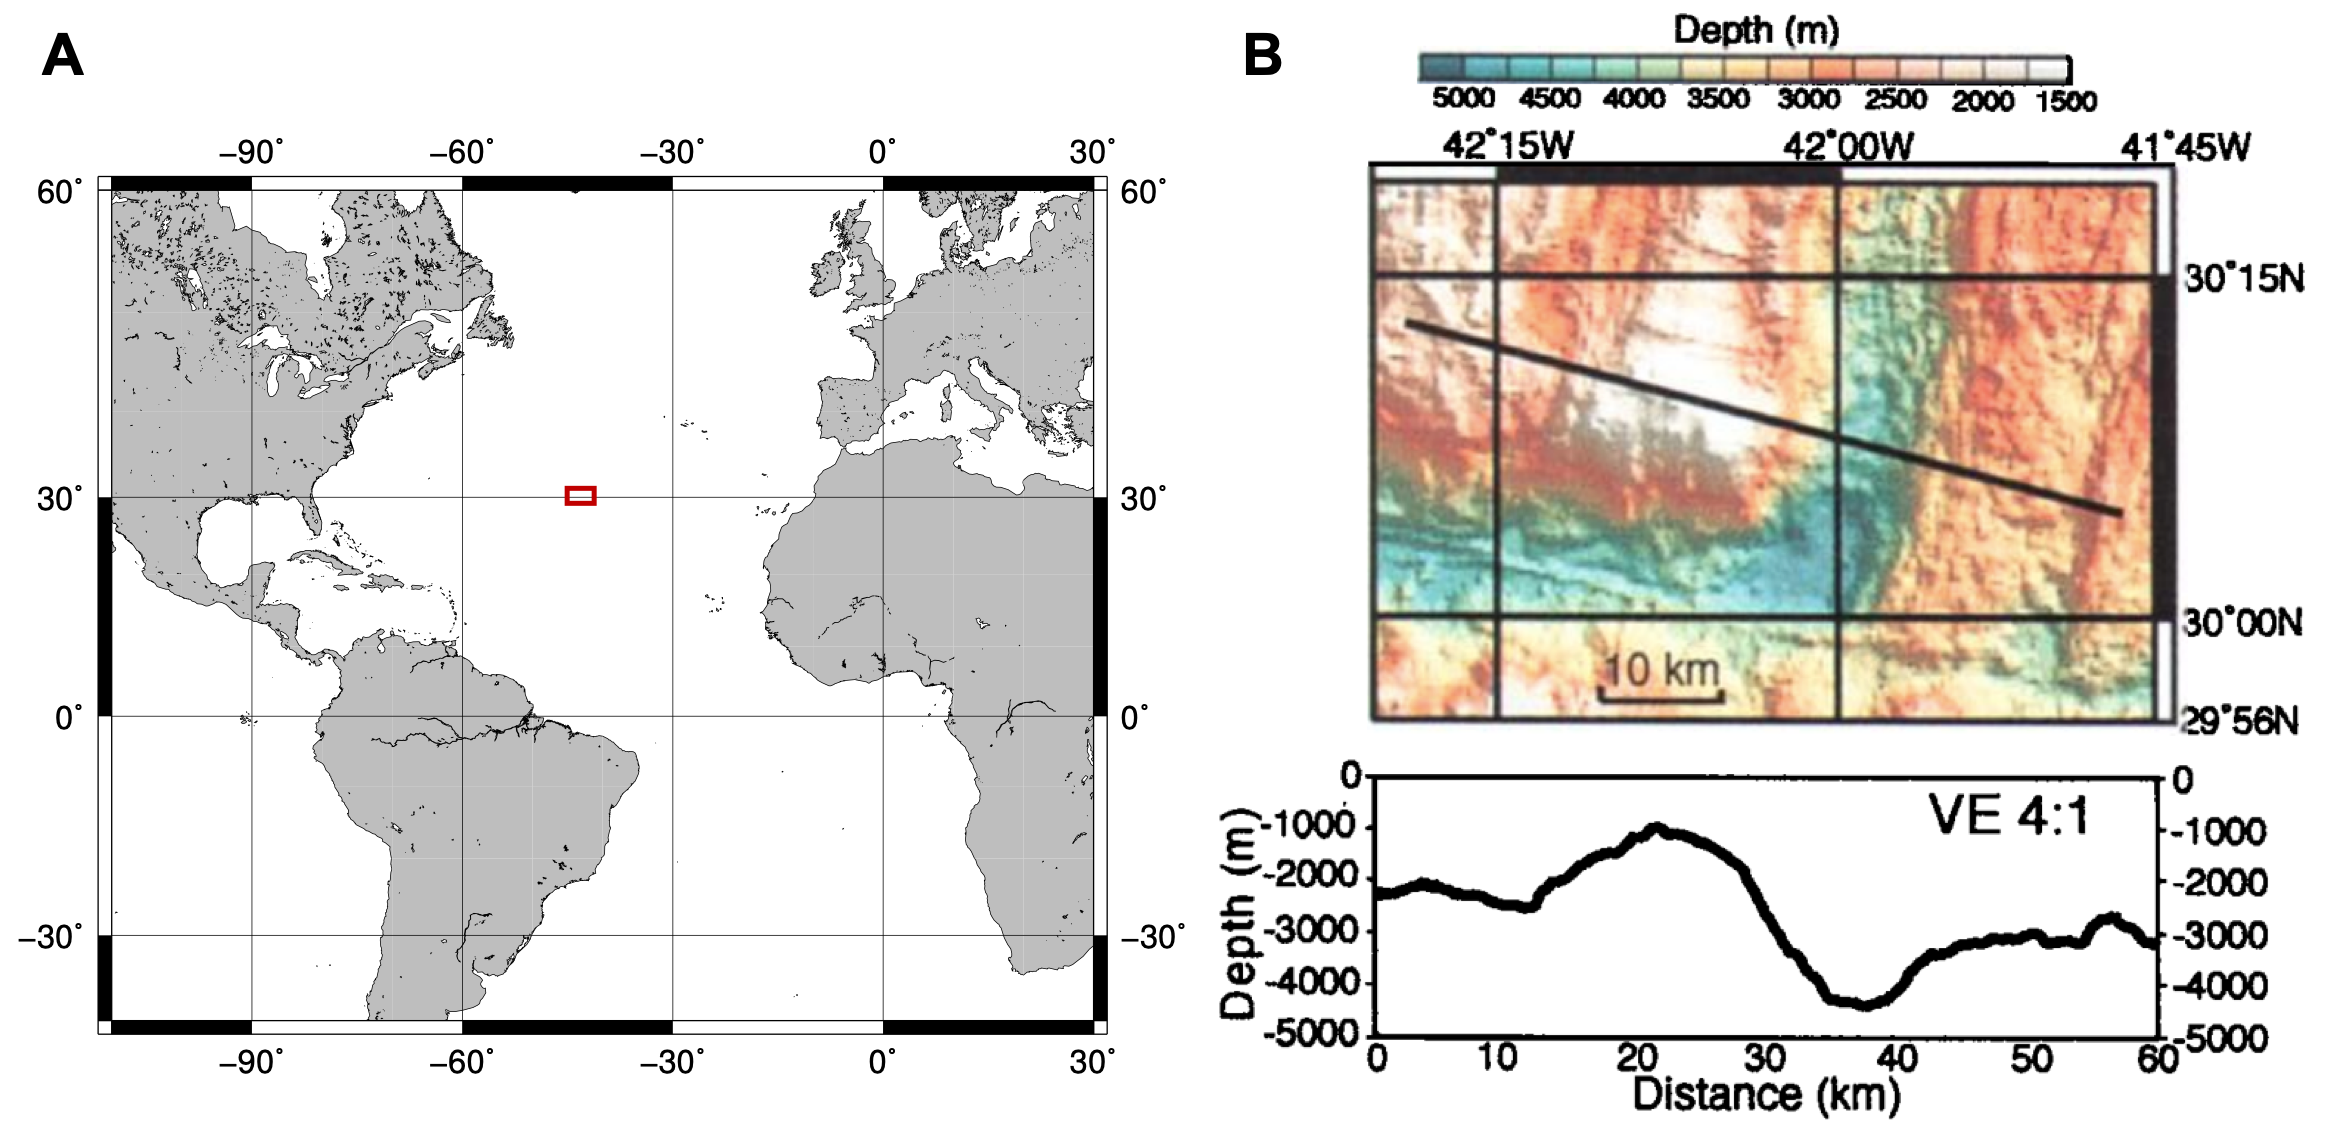
\includegraphics[width=0.9\linewidth,trim=4 4 4 4,clip]{./figs/occ.png}
	\caption{\textbf{A.} The location of Mid-Atlantic Ridge (MAR). Red box indicates the area shown in \textbf{B}. \textbf{B.} Multibeam bathymetry data of MAR gridded at 200m spacing (RIDGE Multibeam Synthesis). Topographic profile along estimated direction of spreading shows detachment fault. From \citet{Lavier2000}}
	\label{fig:occ}
\end{figure}
%

Numerical models with M implemented successfully reproduce the main characteristics of intermediate- and slow-spreading ridges~\citep{Buck2005}.
In the case of M = 0.95, the model produces a symmetric pattern of small-offset faults, producing a bathymetric profile similar to abyssal hills around the Southeast Indian Ridge (Figure \ref{fig:mfactor}A). 
The OCC formation is well reproduced in the model for M = 0.5 \citep{Buck2005}. In their model, two large offset faults form on one side, and a series of small faults form on the other side. Lithospheric stretching creates conjugate normal faults at the spreading center initially. Only one branch survives on one side of the ridge, eventually evolving into a detachment fault, while short-lived new faults semi-regularly form on the opposite side. The resultant bathymetric profile resembles that of the slow-spreading Mid-Atlantic Ridge (Figure \ref{fig:mfactor}B).
%
\begin{figure}[!htb]
	\centering
	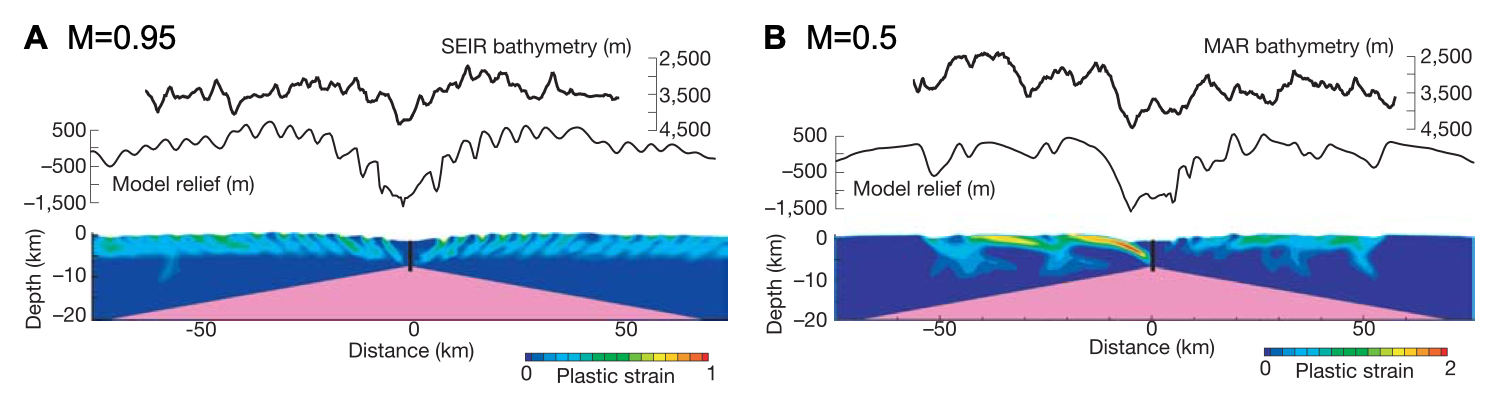
\includegraphics[width=0.65\linewidth,trim=4 4 4 4,clip]{./figs/fig1.png}
	\caption{\textbf{A.} Plastic strain distribution and surface relief from the numerical model with M = 0.95. High plastic strain represents shearing on faults and the bathymetric profile across the Southeast Indian Ridge (SEIR) is shown for comparison. \textbf{B.} Same as \textbf{A} but for M = 0.5. A bathymetric profile from the Mid-Atlantic Ridge (MAR) is shown for comparison. From \citet{Buck2005}}
	\label{fig:mfactor}
\end{figure}

%\section{Numerical approach}
%\note[EC]{Let's reorganize ``Numerical approach'' as follows: Governing equations, Numerical methods for approximate solution. Then, ``Model Setup'' becomes a new (sub-)section.}

%\section{Governing equation}
%mass balance equation
%\begin{align}
% \frac{\partial \rho}{\partial t} + \nabla \cdot (\rho \mathbf{v}) = 0
%\end{align}
%
%linear momentum balance equation
%\begin{align}
%\nabla \cdot \boldsymbol{\sigma} + \rho \mathbf{b} = \rho \frac{D \mathbf{v}}{Dt}
%\end{align}
%
%energy balance equation
%\begin{align}
%\rho C_{p} \frac{\partial T}{\partial t} = k \nabla^2 T
%\end{align}
%
%and constitutive equation for a non-Newtonian fluid
%

\section{Numerical method for governing equations}
FLAC (Fast Lagrangian Analysis of Continua)~\citep{Cundall1982, Poliakov1993, Lavier2002} solves the equation of linear momentum conservation:
\begin{align}
\rho \frac{D \mathbf{v}}{Dt} = \nabla \cdot \boldsymbol{\sigma} + \rho \mathbf{b},
\end{align}
where $D/Dt$ is the material time derivative, $\rho$ is density, $\mathbf{v}$ is velocity, $\boldsymbol{\sigma}$ is the Cauchy stress tensor, and $\mathbf{b}$ is body force. %%
%energy balance equation
FLAC also solves the energy balance equation,
\begin{align}
\rho c_{p} \frac{D T}{D t} = \nabla \cdot ( k \nabla T)
\end{align}
where $c_{p}$ is specific heat capacity at constant pressure, $T$ is temperature, and $k$ is a coefficient of thermal conductivity. 
%
%\noindent for a visco-elastic-plastic continuum in 2-D Cartesian geometry. 
These equations are converted to the respective weak forms and finite element method for linear triangular elements is employed to compute approximate solutions. The acceleration term in the momentum conservation equation is integrated explicitly in time for updated velocities, which in term are used for updating strain rates, strain and stress. The updated variables are used to determine the acceleration as the sum of the internal and external forces for the next time step. The energy balance equation is similarly integrated to update temperature. The FLAC code that I used for this study is available at \url{https://github.com/heec12/Mscthesis}. The input parameter files necessary for reproducing the results presented in this study are available in the same repository.

Materials in my mid-ocean ridge models are assumed to be elasto-visco-plastic. In this rheology, the brittle behavior is modeled by strain-weakening elasto-plasticity and the ductile behavior is modeled by Maxwell visco-elasticity. 
For visco-elastic deformation, the linear Maxwell viscoelastic model is adopted, in which strain rates are assumed to be the sum of elastic and viscous strain rates.
\begin{align} \label{srate}
  \dot{\epsilon} &=  {\dot{\epsilon}}_{els} +  {\dot{\epsilon}}_{vis} \\
                        &= \frac{ \dot{\sigma}}{k} + \frac{\sigma}{\eta}
\end{align}
where $\dot{\epsilon}$ is strain rate, $\sigma$ is stress, $k$ is constant, and $\eta$ is viscosity.
%

Viscosity is determined by the dry diabase power law rheology~\citep{Kirby1987, Chen1990}.
\begin{align} \label{Visc}
 \eta = \frac{1}{4} \bigg( \frac{4}{3A} \bigg)^{1/n} \dot{\epsilon}^{(1/n)-1} \exp\bigg(\frac{Q}{nRT}\bigg)
\end{align}
where $n$ is the power-law exponent, $A$ is the pre-exponential factor that depends on temperature and pressure, $Q$ is the quality factor, $R$ is the universal gas constant, and $T$ is temperature.
%

Plastic yielding is controlled by the strain-weakening Mohr-coulomb plasticity model. In this model, the yield stress is determined as
\begin{align}
 \tau = \mu \sigma_n + C,
\end{align}
where $\tau$ and $\sigma_{n}$ are shear and normal stress, $\mu$ is friction coefficient and $C$ is cohesion.
%
Strain weakening is realized by decreasing cohesion with the total accumulated plastic strain while friction coefficient is assumed to be constant~\citep{Poliakov1998}. In this study, cohesion decreases linearly from its initial value 44 MPa to the minimum value of 4 MPa.
%
\begin{table}[h!]
	\centering
	\caption{Summary of model parameters}
	\label{tab:modelparams}
	\begin{tabular}{cccc}
		\toprule
		Variable & Description & Value & Units\\
		\midrule
          	$\lambda$ & Density & 3300 & $kg/m^3$\\
	        n & From Eq \ref{Visc} & 4.7 & \\
	        A & From Eq \ref{Visc} & 190 & \\
	        E & Activation energy & 4.85e+5 & $kJ/mol$ \\
	        $\lambda$ & 1st Lam\'e parameter & 12 & GPa\\
	        $G$ & Shear modulus & 12 & GPa\\
	        $C_{max}$ & Maximum cohesion & 44 & MPa\\
	        $C_{min}$ & Minimum cohesion & 4 & MPa\\
		\bottomrule
	\end{tabular}
\end{table}
%

\section{Model Setup}
The model domain is rectangular with a ridge axis at the center  (Fig.~\ref{fig:modelsetup}). All the models have 60 km wide and 20 km deep domain sizes with a grid of 0.5 $\times$ 0.5 km, each rectangular element of which is subdivided into triangles. At the top boundary, I apply stress-free surface.
%\annote[EC]{a hydrostatic pressure of XX MPa, corresponding to XX km-thick seawater layer}{Fill out the missing info.}. 
The bottom boundary has the Winkler foundation, which is normal stress that equal the local lithostatic pressure.
%
\begin{figure}[!htb]
	\centering
	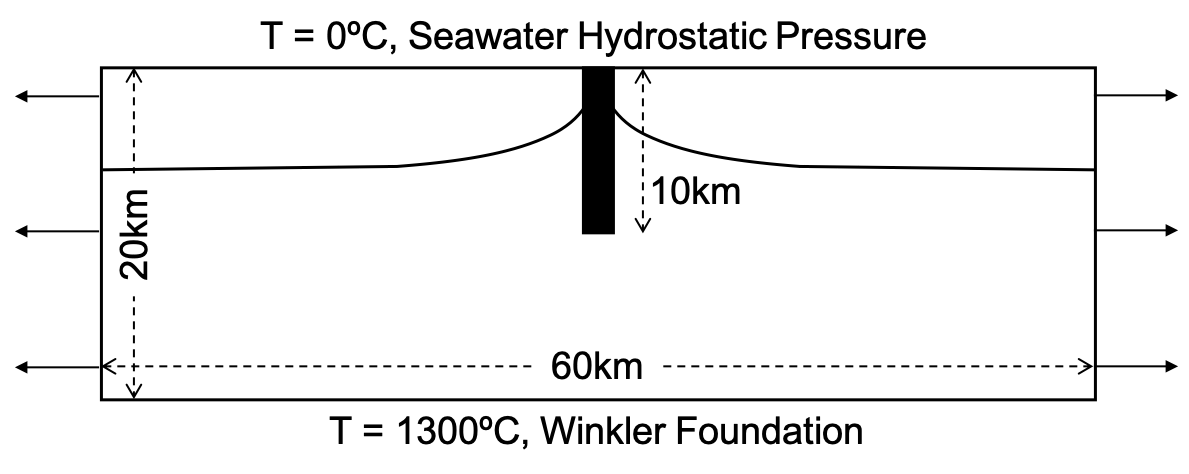
\includegraphics[width=0.8\linewidth,trim=8 8 8 8,clip]{./figs/modelsetup.png}
	\caption{Model setup used for numerical simulations of mid-ocean ridge system. For both velocity- and force-driven model, same initial and thermal boundary conditions are applied.}
	%\note[EC]{Show and state the directions of your x and y axis and the origin at the top center of the domain. Without this info, later velocity plots and distance axis wouldn\rq{}t make sense immediately.}}
	\label{fig:modelsetup}
\end{figure}
%

Building on this common basis, I explore how oceanic plates grow when plate motions are driven by forces applied on the boundary rather than by prescribed kinematics. Three cases with an increasing order of complexity are considered.

\subsection{Case I: Kinematic models}

Plate motions are driven by prescribed velocities on the left and right boundaries at a rate of 2.5cm/yr. The purpose of this traditional approach is to verify that the faulting modes are reproduced as in the previous studies \citep{Buck2005,Tucholke2008}.

\subsection{Case II: $(\boldsymbol{F_{res}})_x \mathbf{=0}$ models}

Plate motions are assumed to occur as a result of the balance between three forces acting on plates (Figure \ref{fig:forcescheme}): (1) Boundary force ($\mathbf{F}_{bdy}$) applied at the two side boundaries of lithosphere; (2) brittle force ($\boldsymbol{F}_{brt}$) arising as lithophere is elastically stretched, creates faults and keeps them active; %or forms faults a counter force to $F_{bdy}$ in the opposite direction; 
and (3) viscous force ($\boldsymbol{F}_{vis}$) required for lithosphere to drag asthenosphere along. 
%Additionally, the force from faulting and its evolution is called fault force ($\boldsymbol{F_{fault}}$). 
For later purposes, the sum of the latter two is termed as an internal force ($\boldsymbol{F}_{int}$). Then, residual force ($\boldsymbol{F}_{res}$) can be defined as the sum of $\boldsymbol{F}_{bdy}$ and $\boldsymbol{F}_{int}$:
%
\begin{align} \label{Fres}
\mathbf{F}_{res} & = (\mathbf{F}_{brt} + \mathbf{F}_{vis}) + \mathbf{F}_{bdy} \\
 & = \mathbf{F}_{int} + \mathbf{F}_{bdy}.
\end{align}
%
\begin{figure}[!htb]
	\centering
	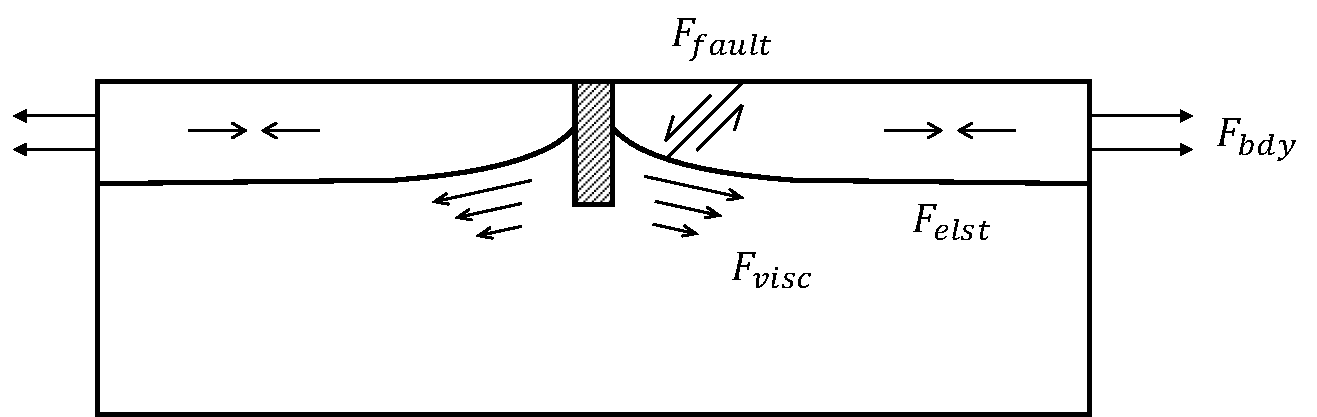
\includegraphics[width=0.7\linewidth]{./figs/force.pdf}
	\caption{Schematic illustration of the internal forces and boundary forces apply to the model.}
	\label{fig:forcescheme}
\end{figure}

Since $(\boldsymbol{F}_{int})_{x}$ is only a response to the boundary force and it is $(\boldsymbol{F}_{res})_{x}$ that determines how lithosphere accelerates, I control the magnitude of $(\boldsymbol{F}_{res})_{x}$ to initiate the motion of plates, which are at rest in the beginning, and maintain their speeds at a target value. Since $(\boldsymbol{F}_{int})_{x}$ would vary in time as faults grow or other changes occur in lithosphere and asthenosphere, setting $(\boldsymbol{F}_{res})_{x}$ %, the sum of $F_{bdy}$ and $F_{int}$, 
to be a certain value implies that $(\boldsymbol{F}_{bdy})_{x}$ is automatically adjusted such that the sum with $(\boldsymbol{F}_{int})_{x}$ becomes the value. The boundary forces are in practice applied as traction (i.e., surface force per area) in my 2D models with the third dimension assumed to have unit length. The code internally performs the surface integral of tractions to compute boundary forces.

The magnitude of the horizontal component of the residual force, $(\boldsymbol{F}_{res})_{x}$ is initially zero but linearly increases with time until plate spreading rate reaches a desirable value. When the plate speed reaches 2.5 cm/yr, I set the magnitude of $(\boldsymbol{F}_{res})_{x}$ to be zero in order to maintatin the velocity of the plate.

Abrupt application of the residual force often causes the faults to form near the side walls rather than at the spreading center.
% the mean plate speed quadratically
To avoid such an undesirable boundary failure, I search for an appropriate rate of increasing $(\boldsymbol{F}_{res})_{x}$ by observing where faulting occurs. Rates are in the range of 1 to 1000 Pa/yr (Table \ref{tab:slope}). 1 Pa/yr slope is used for M = 0.5 models, and 10 Pa/yr is used for M= 0.8 models. 
%
\begin{table}[h!]
	\centering
	\caption{Model results of 1Myr of spreading for $(\boldsymbol{F_{res}})_x$ increasing slope ranging from 1 to 1000 Pa/yr with two different M value. Expected model behavior for M=0.5 is a master detachment fault and alternating faulting for M=0.8}
	\label{tab:slope}
	\begin{tabular}{ccc}
		\toprule
		Slope, Pa/yr & M = 0.5 & M = 0.8\\
		\midrule
          	1 & Detachment fault forms 71 Kyrs later & Detachment fault forms 240 Kyrs later\\
		10 & Boundary failure occurs & Alternating faulting mode \\
		100 & Boundary failure occurs & Alternating faulting mode \\
		1000 & Boundary failure occurs & Boundary failure occurs\\
		\bottomrule
	\end{tabular}
\end{table}
%
%Setting $(\boldsymbol{F_{res}})_x$ as a zero after initial phase allow me to examine the expected physical behavior in force boundary applied model. 

\subsection{Case III: Constant ($\boldsymbol{F}_{bdy}$)$_x$ models}

Prescribed $x$ component boundary force, ($\boldsymbol{F}_{bdy}$)$_x$ on the boundaries of lithosphere, are applied on this group of models. The net force resulting at the boundary nodes, $(\boldsymbol{F}_{res})$, is determined as the sum of $\boldsymbol{F}_{bdy}$ and time-evolving $\boldsymbol{F}_{int}$.

I assign to $(\boldsymbol{F}_{bdy})_x$ the value of time-averaged $(\boldsymbol{F}_{int})_x$ %($\overline{(\boldsymbol{F}_{res})_x}$) 
from a Case II model with the same value of M. A Case II model with a desired value of M writes $(\boldsymbol{F}_{int})_x$ values on all the side boundary nodes to a file. Those recorded values of $(\boldsymbol{F}_{int})_{x}$ are then averaged over a time period. When M = 0.5, I simply average $(\boldsymbol{F}_{int})_{x}$ values after the master detachment fault forms until the model ends since no new faults break afterwards.
When M is 0.8, the alternating faulting occurs (Fig.~\ref{fig:faultstage}). I divide the evolution of alternating faulting into three stages: Incipient, mature and terminal. At the incipient stage (Figure \ref{fig:faultstage}A), a fault forms on one side of the ridge axis. The fault heave increases and fault dip decreases as fault grows during the mature stage (Figure \ref{fig:faultstage}B). The terminal stage is characterized by the replacement of the locked fault by a new near-axis fault on the opposite side of ridge axis. The force-averaging period for a M=0.8 model is the time between the snapshot B (149 Kyr) and C (250 Kyr), from the mature stage of the first fault to the incipient stage of the next new fault on the opposite side. 
%
\begin{figure}[!htb]
	\centering
	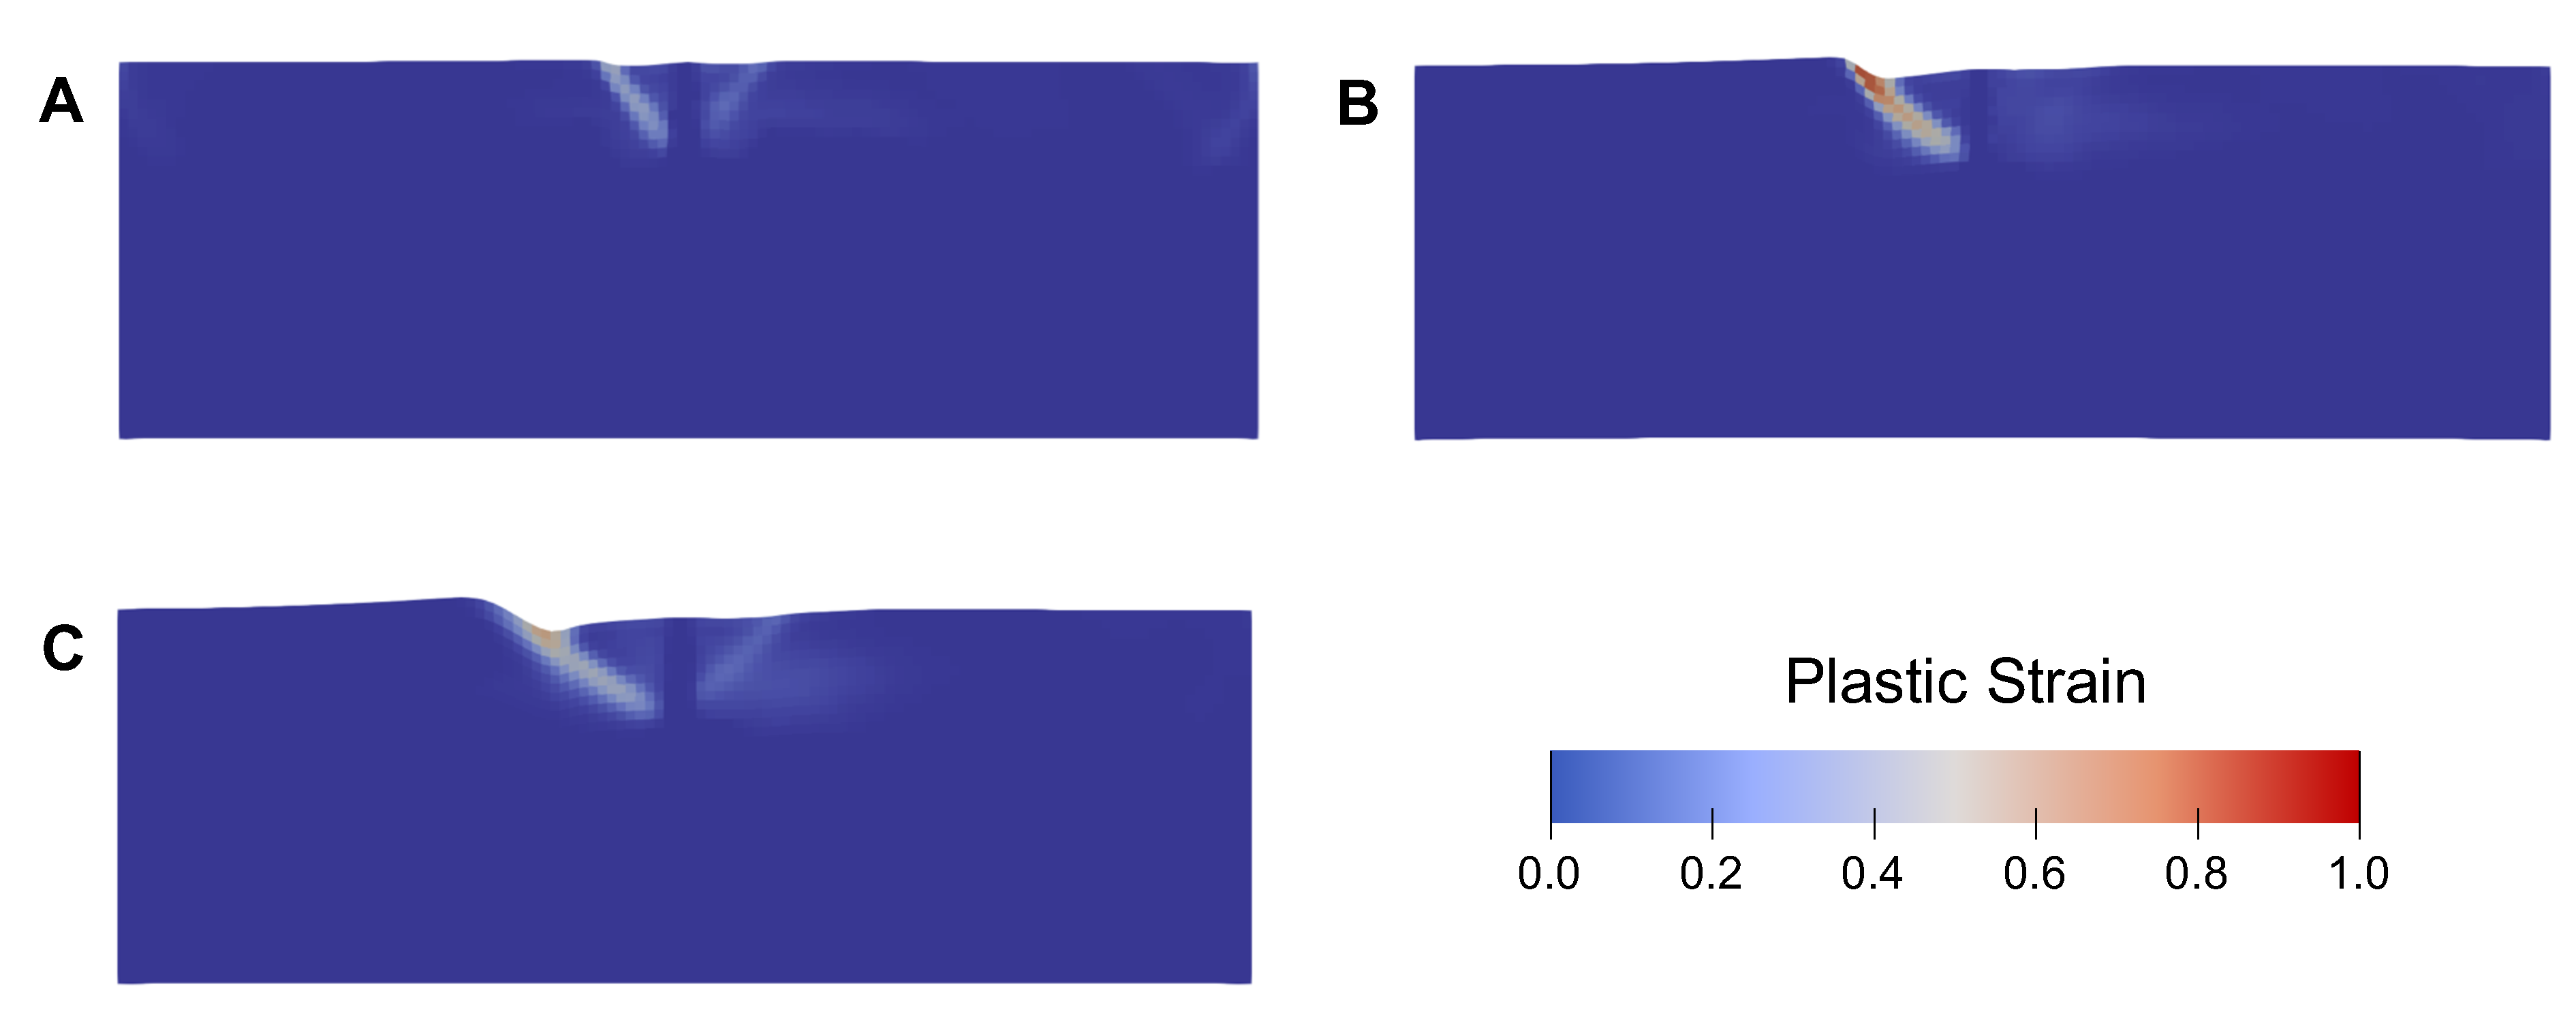
\includegraphics[width=0.9\linewidth]{./figs/fault_stage.pdf}
	\caption{Snapshots of the kinematic model (M = 0.8) representing stages of the fault evolution. The fault evolution can be divided as three stages. \textbf{A.} Incipient stage: new fault occurs on left side of the ridge axis. \textbf{B.} Mature stage: fault heave increases and fault dip decreases as fault grows. \textbf{C.} Terminal stage: fault becomes inactive and is replaced by a new-near axis fault on the other side of ridge axis.}
	\label{fig:faultstage}
\end{figure}

$(\boldsymbol{F_{res}})_x$ is applied only to the nodes in the brittle state, in which I assume temperature is lower than 600 $^\circ$C \citep[e.g.,][]{Violay2012}. Assuming that the ductile mantle is only passively pulled up beneath the spreading center and dragged along by the brittle lithosphere, I set ($\boldsymbol{F}_{res}$)$_x$ of the ductile parts of the side boundaries to be zero. This treatment is equivalent to assuming that the boundary force is perfectly balanced with the viscous resistance on the ductile portions of the boundaries. %Most of tectonic activities have been shown to be a consequences of plate motions. Therefore, I apply the force only acting on brittle plates and let $(\boldsymbol{F_{bdy}})_x$ as a zero.

\chapter{Results}

\section{Kinematic models}

The kinematic models reproduce the faulting modes reported in the previous studies. When M is 0.5, a normal fault forms by 0.1 Myr and remains active over the entire duration of the model, 1 Myr, producing an oceanic core complex (Figure \ref{fig:kfault}A). When M is 0.8, a normal fault form by 0.1 Myr but it locks over the next 0.1 Myr and eventually being replaced by another fault forming on the opposite side. Going through the same sequence of events with the first fault, the second fault is replaced by the third one by 0.4 Myr. The alternating faulting continues until the model ends after 1 Myr (Figure \ref{fig:kfault}B).
%
\begin{figure}[!htb]
	\centering
	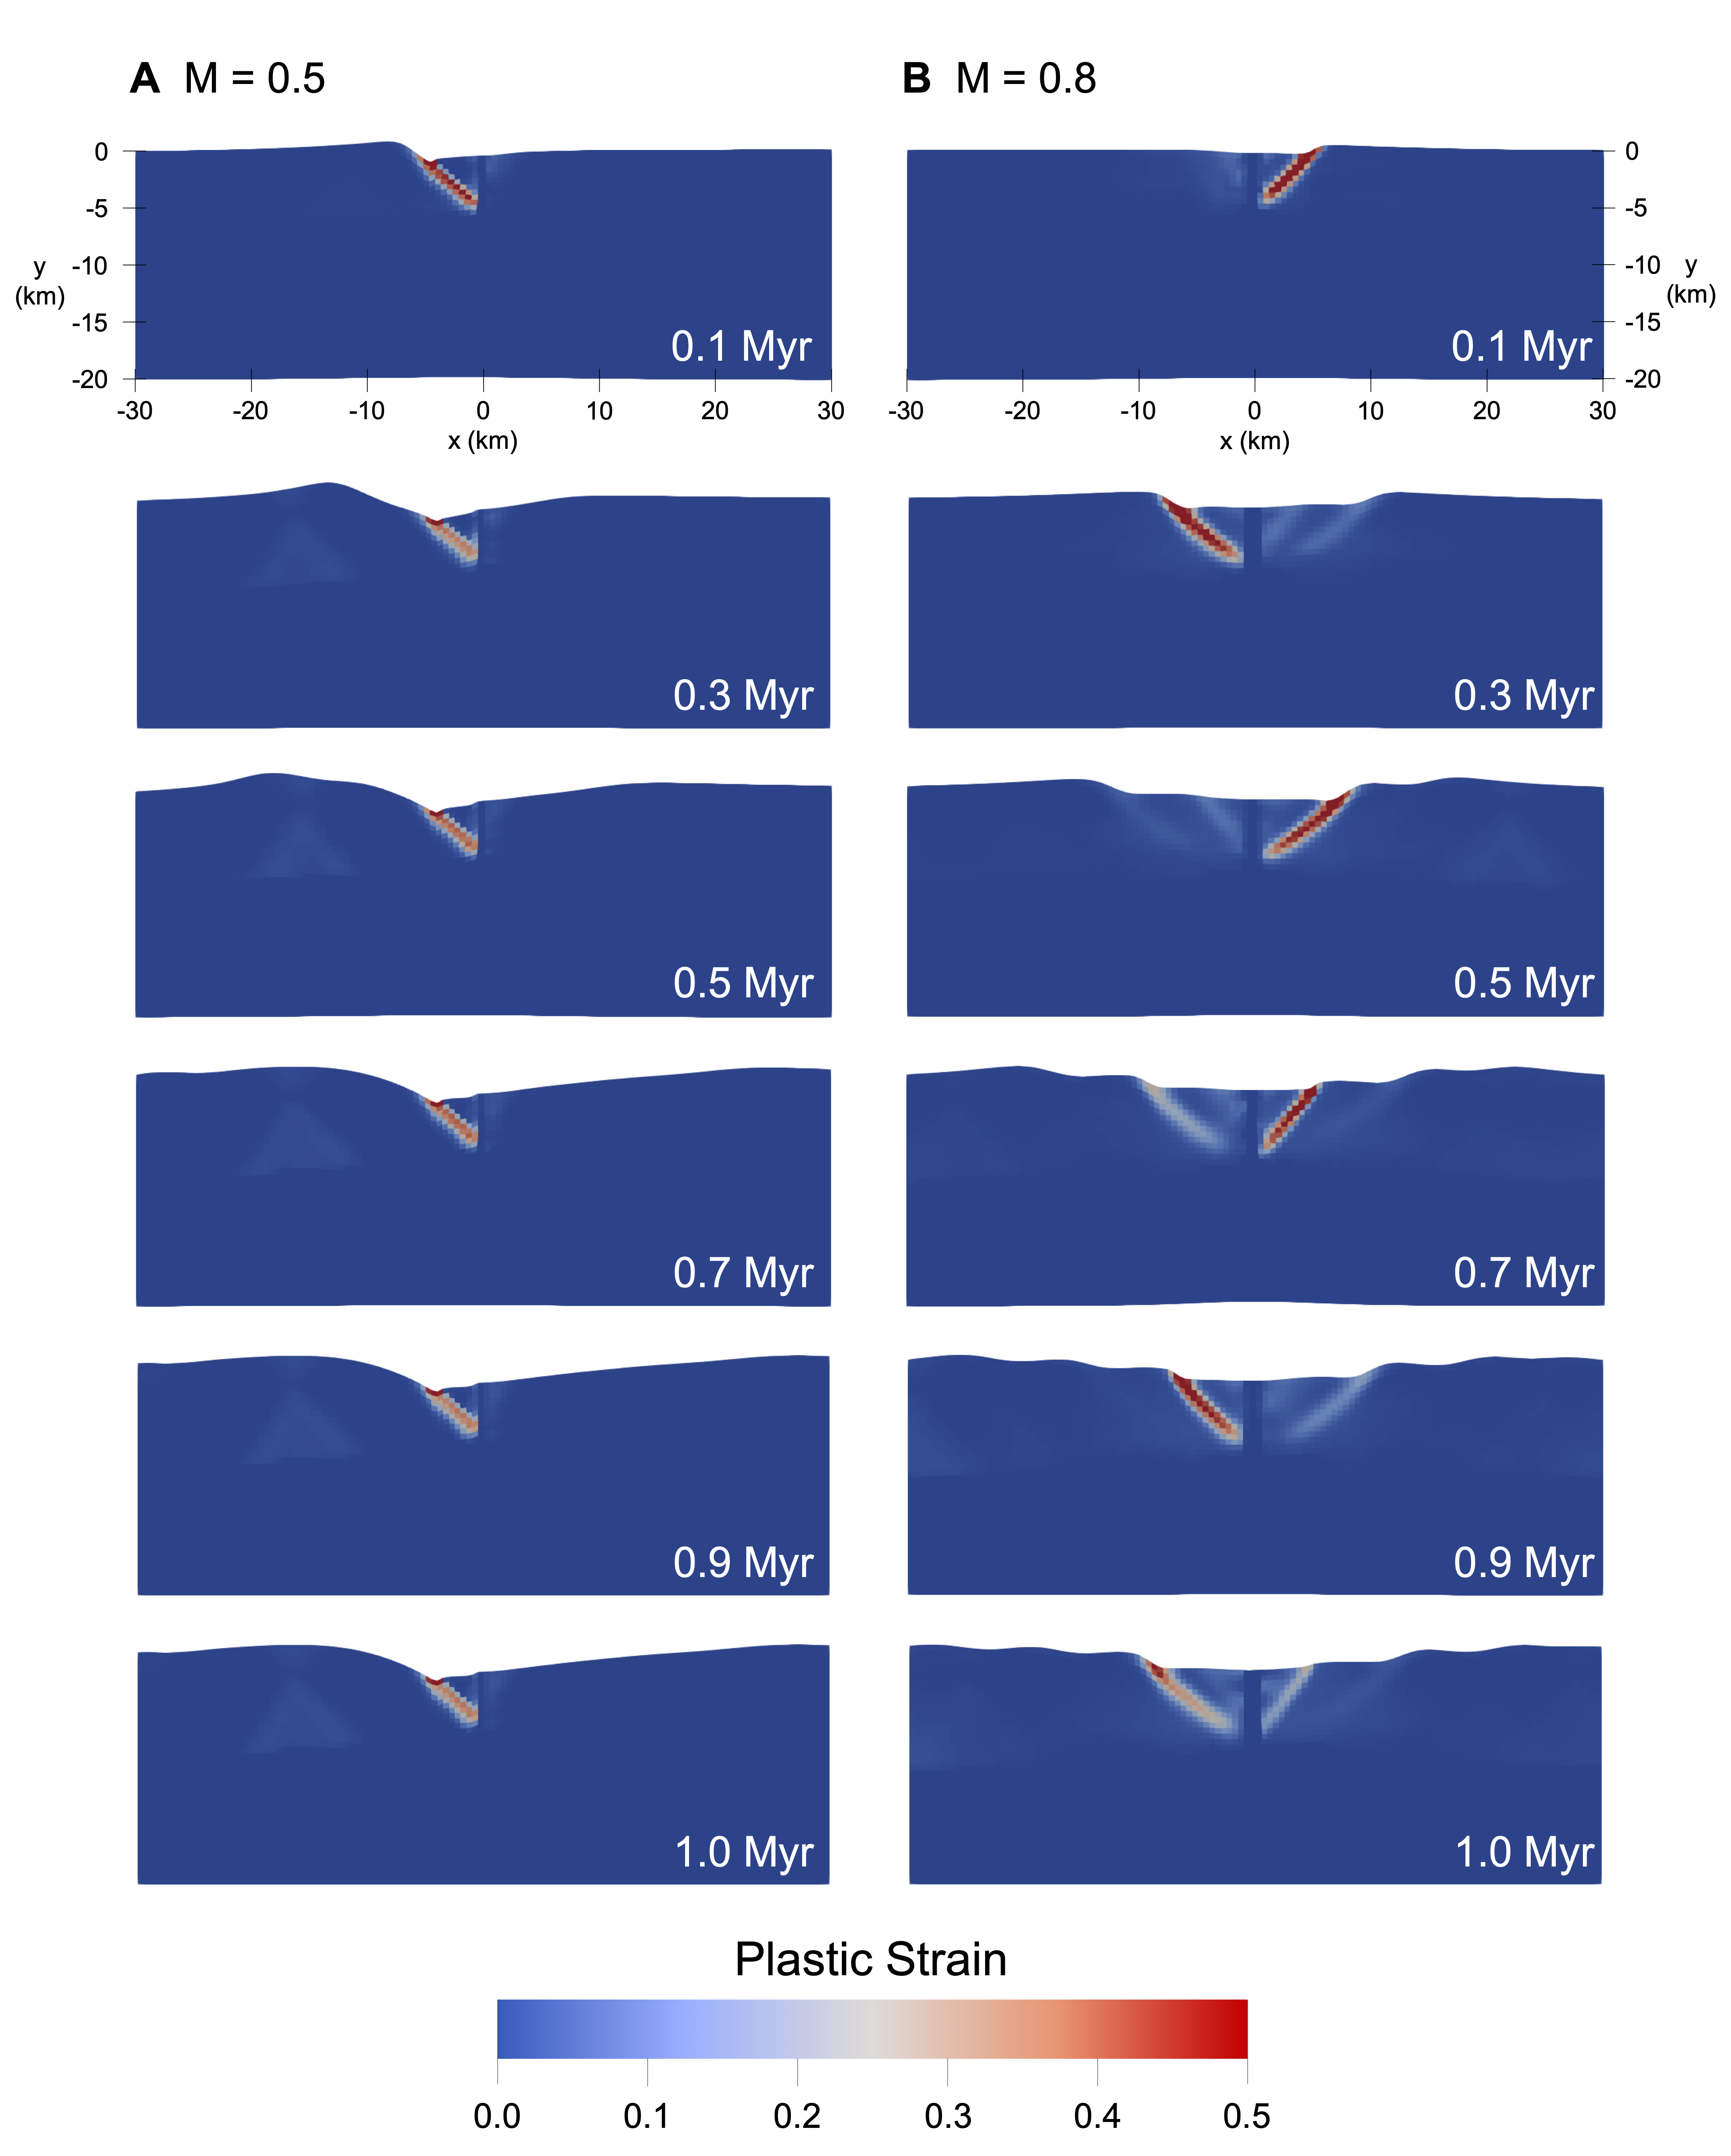
\includegraphics[width=0.74\linewidth,trim=20 30 20 20,clip]{./figs/kfault.png}
	\caption{ \textbf{A.} Snapshots of plastic strain distribution in the kinematic model with M = 0.5 over 1 Myr at 0.2 Myr interval. Bands of localized plastic strain represent faults. \textbf{B.} Same as \textbf{A} but for M = 0.8.}
	\label{fig:kfault}
\end{figure}

Mean horizontal velocity of each plate ($\overline{\boldsymbol{v}}_{x}$) is defined as averaged $x$ component of the nodal velocities on the top surface nodes $\sim$15 km away from the ridge axis. The central 30 km-wide area is excluded from averaging to eliminate faulting effects. 
%To avoid aliasing, I printed $\overline{\boldsymbol{v}}_{x}$ values at every time steps. In this way, I verified that the abnormal peaks came from the remeshing events and obtained putative plate velocity. 
FLAC does remeshing \citep{Lavier2002} when deformations being simulated distort elements exceeding twice longer than the original length. Interpolation of variables of the distorted mesh onto a new one results in out-of-balance forces at the nodes and produces artificial accelerations. The raw value of $\overline{\boldsymbol{v}}_{x}$ includes the noise produced due to these artificial accelerations. To filter them out and see $\overline{\boldsymbol{v}}_{x}$ more clearly, I applied a second order Butterworth low-pass filter (Figure \ref{fig:filter}) to reconstruct the mean speed time series using only frequencies lower than 6.34 $\times 10^{-10}$ Hz.
%
\begin{figure}[!htb]
	\centering
	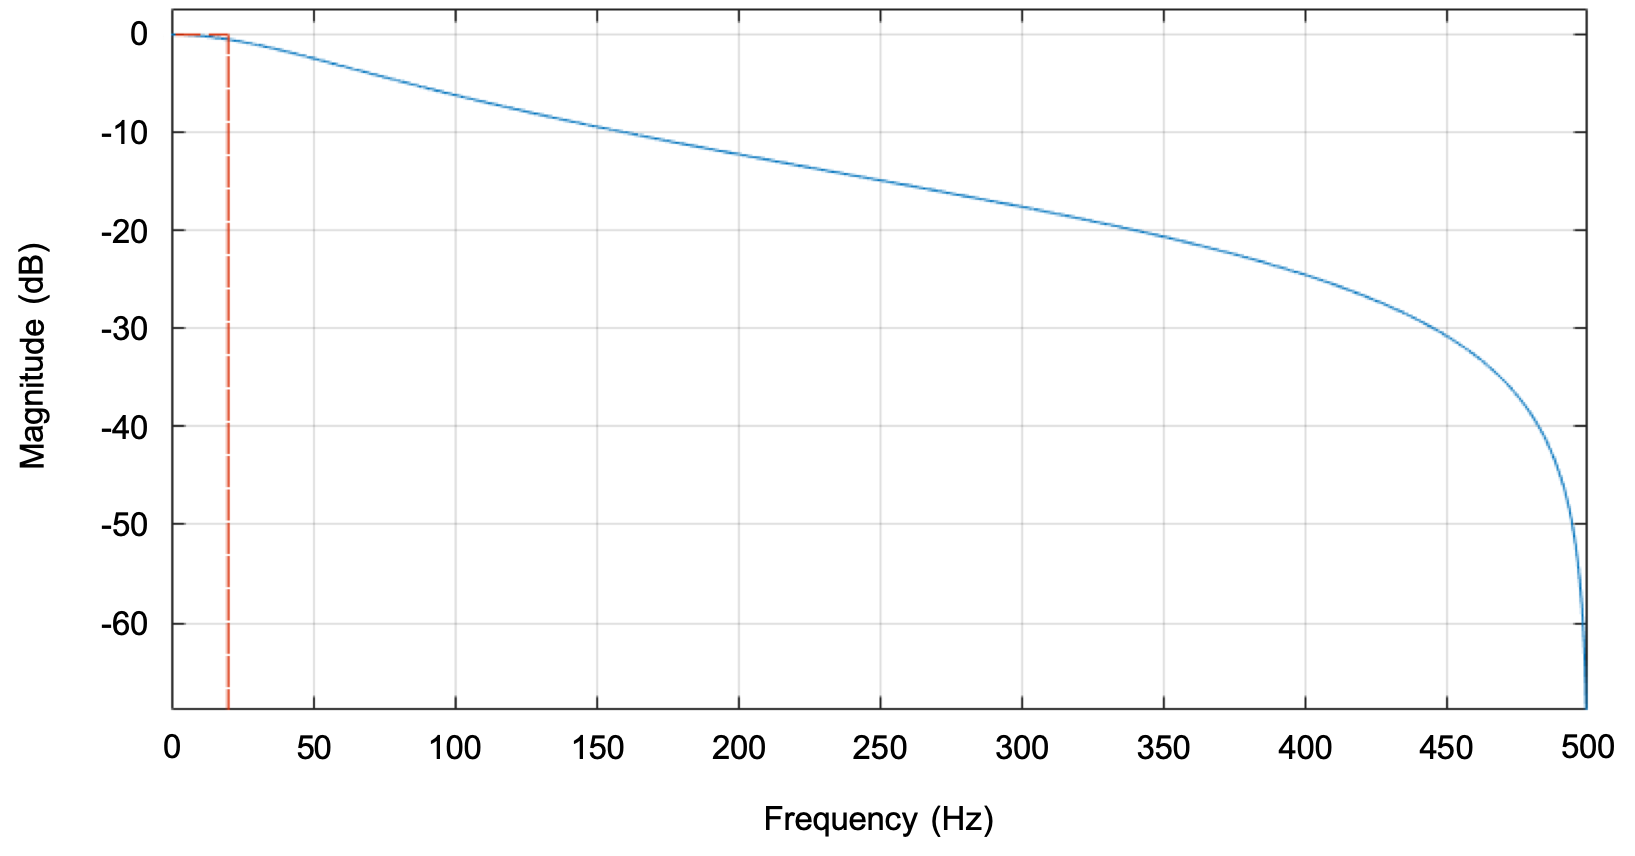
\includegraphics[width=0.8\linewidth,trim=4 4 4 4,clip]{./figs/filter.png}
	\caption{Magnitude response of designed second order Butterworth low-pass filter. In this filter, the frequencies under 20 $\times$ 1/Kyr, surrounded with red lines, are in the pass band and the higher frequencies are in the stop band.}
	\label{fig:filter}
\end{figure}

Mean horizontal velocity of each plate ($\overline{\boldsymbol{v}}_{x}$) in the kinematic models is constant as expected. 
When M = 0.5, $\overline{\boldsymbol{v}}_{x}$ remain constant at 2.50 cm/yr on left-side plate and 2.55 cm/yr on right-side plate (Figure \ref{fig:kmhv}A). Also, at M = 0.8, $\overline{\boldsymbol{v}}_{x}$ remain constant at 2.55 cm/yr on both sides of plate until the model ends (Figure \ref{fig:kmhv}B). %Filtered $\overline{\boldsymbol{v}}_{x}$ is plotted as a red line.
%
\begin{figure}[!htb]
	\centering
	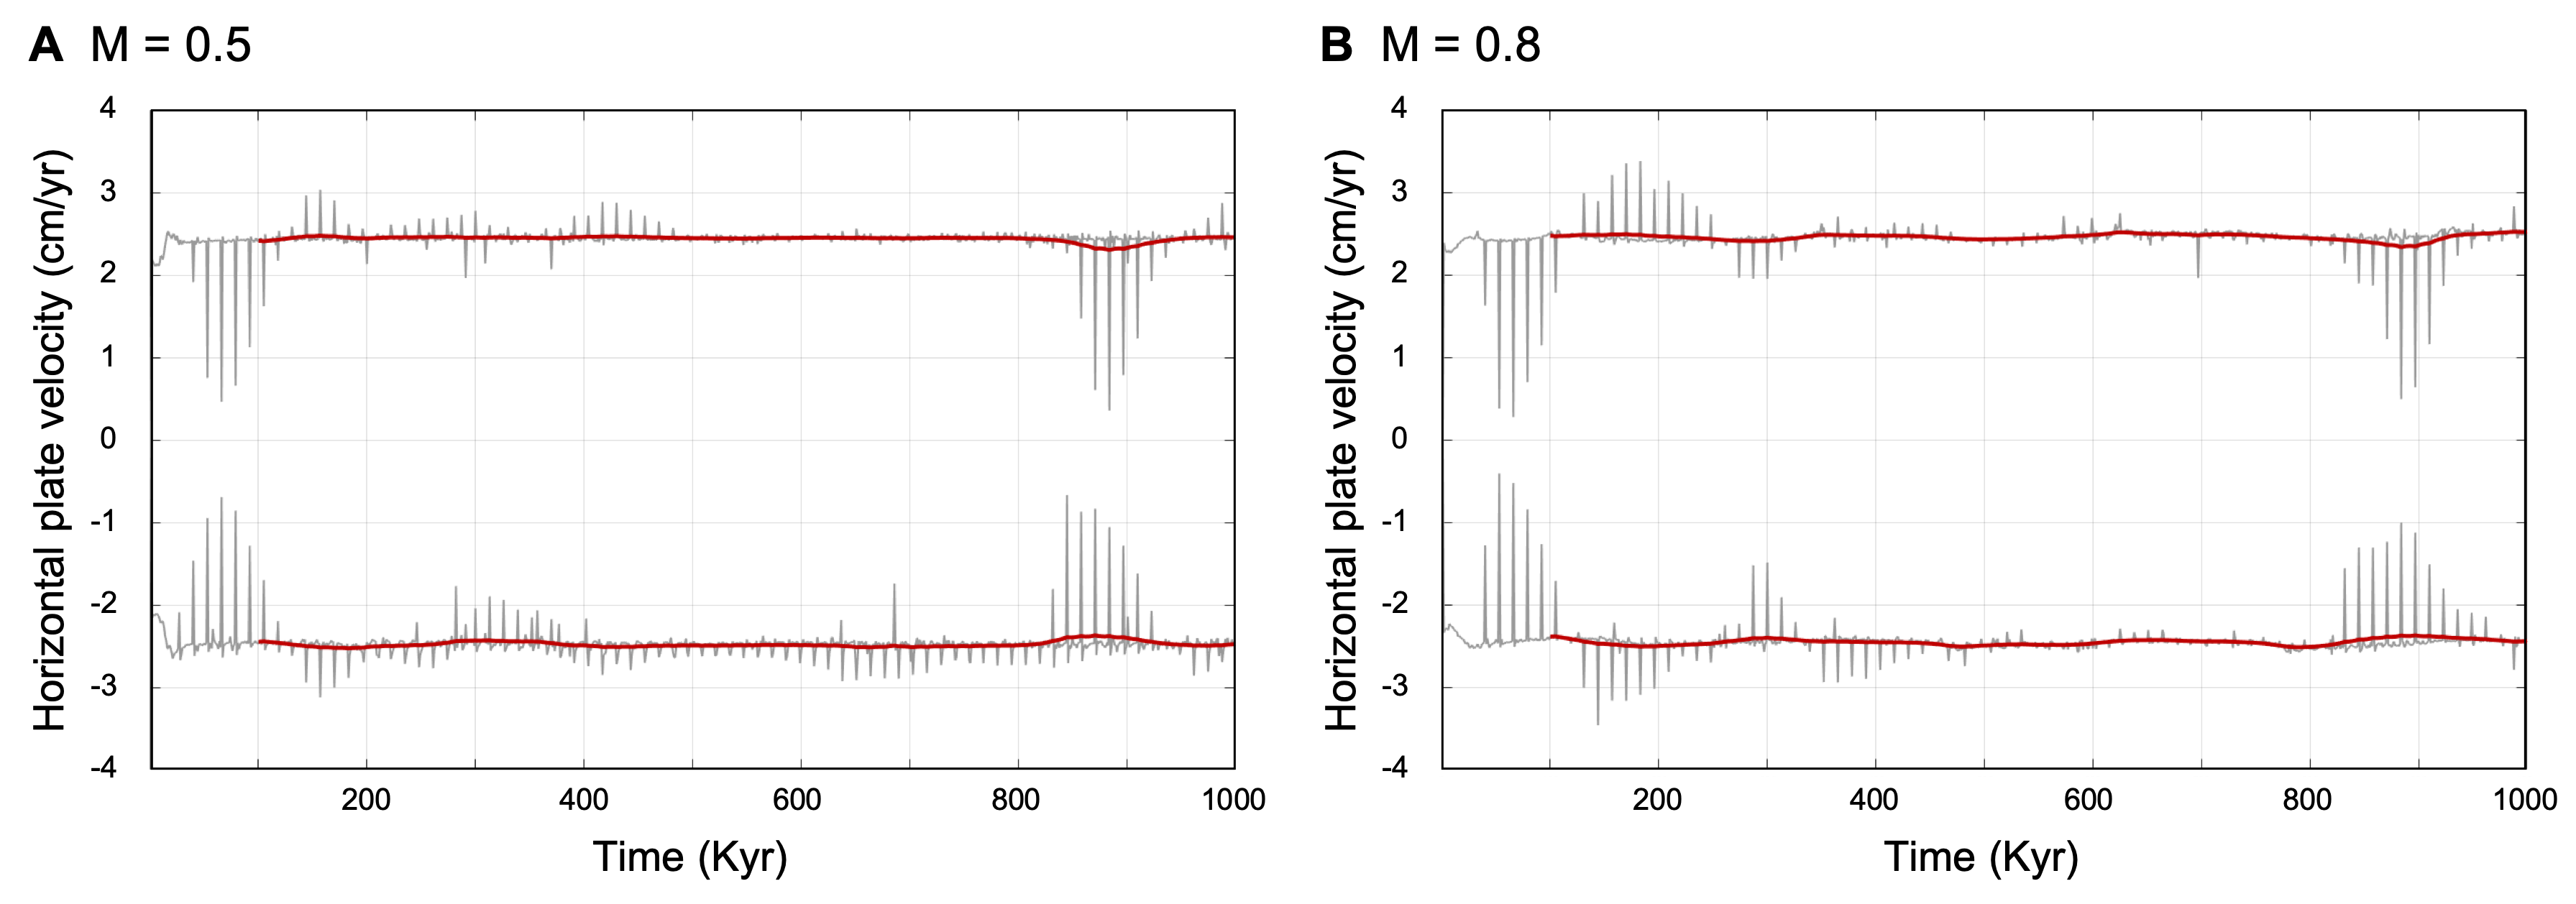
\includegraphics[width=0.98\linewidth,trim=4 4 4 4,clip]{./figs/kmhv.png}
	\caption{\textbf{A.} (Up) Mean horizontal plate velocity obtained from M=0.5 kinematic model results. Red lines are filtered velocity. The positive values represent the right-moving plate and the negative values represent the left-moving plate. (Down) Absolute value of filtered velocity. Blue line is left-moving plate and red line is right-moving plate. \textbf{B.} Same as \textbf{A} but for M = 0.8.}
	\label{fig:kmhv}
\end{figure}
%However, the velocity-driven models do not show the observed non-uniform plate velocity by simply changing magmatism at the spreading center.

\section{$(\boldsymbol{F_{res}})_x=0$ models}

This condition represents the hypothetical state where $\boldsymbol{F}_{bdy}$ is adjusted such that it perfectly counteracts $\boldsymbol{F}_{int}$ making $\boldsymbol{F}_{res}$ equal to zero all the time. %Simplest condition in force-driven models. 
Since the net residual force is zero on the side boundaries, the models under this condition show constant plate velocity as expected for a motion with zero acceleration.

Faulting styles in the models with this force boundary condition show the same correspondence with M values as in the previous studies \citep{Buck2005,Tucholke2008}. One master detachment fault creates an OCC when M = 0.5 (Figure \ref{fig:f0fault}A) and a series of small offset normal faults, forming alternatingly on both sides of the ridge axis, produce abyssal hills when M = 0.8(Figure \ref{fig:f0fault}B).
%
%\begin{figure}[!htb]
%	\centering
%	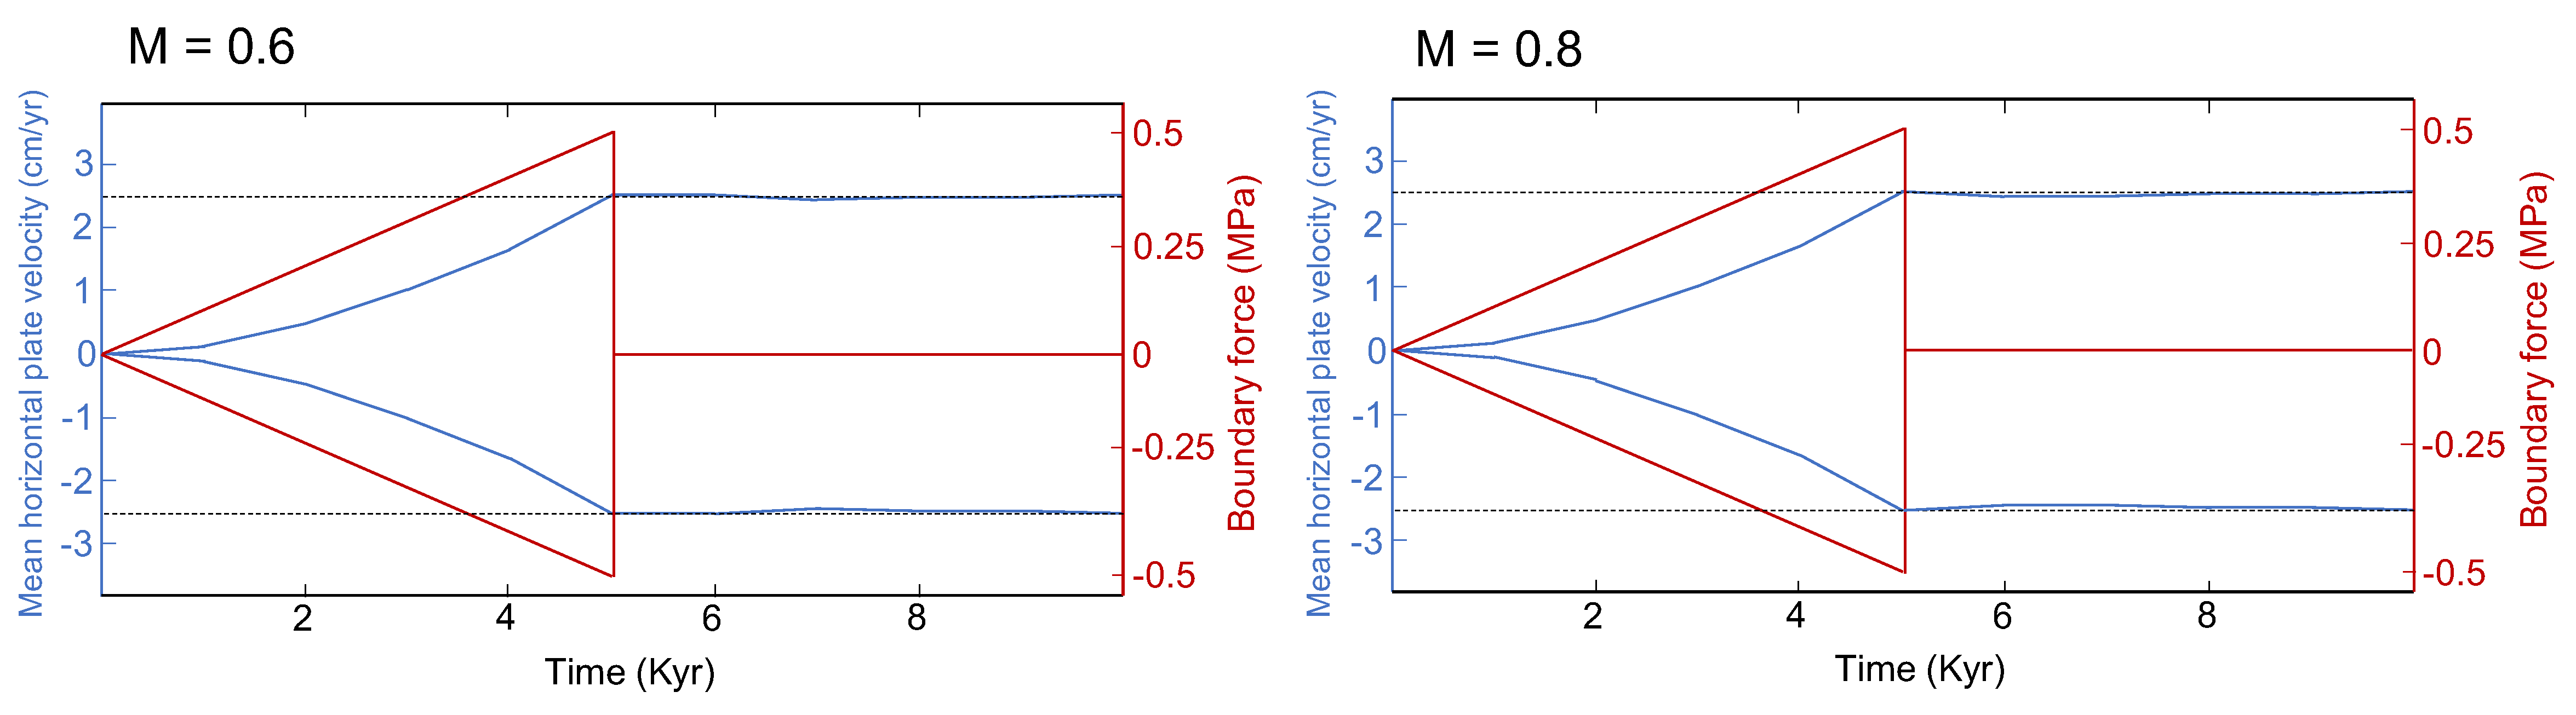
\includegraphics[width=0.99\linewidth]{./figs/force0.pdf}
%	\caption{Velocity and boundary force($(\boldsymbol{F_{bdy}})_x$) as a function of time. $(\boldsymbol{F_{bdy}})_x$ increases linearly with time until the plate speed quadratically increase to 2.5 cm /yr. At that moment, $(\boldsymbol{F_{bdy}})_x$ is reduced to zero so that the horizontal plate velocity is maintained at the target value of 2.5 cm/yr.}
%	\label{fig:force0}
%\end{figure}
\begin{figure}[!htb]
	\centering
	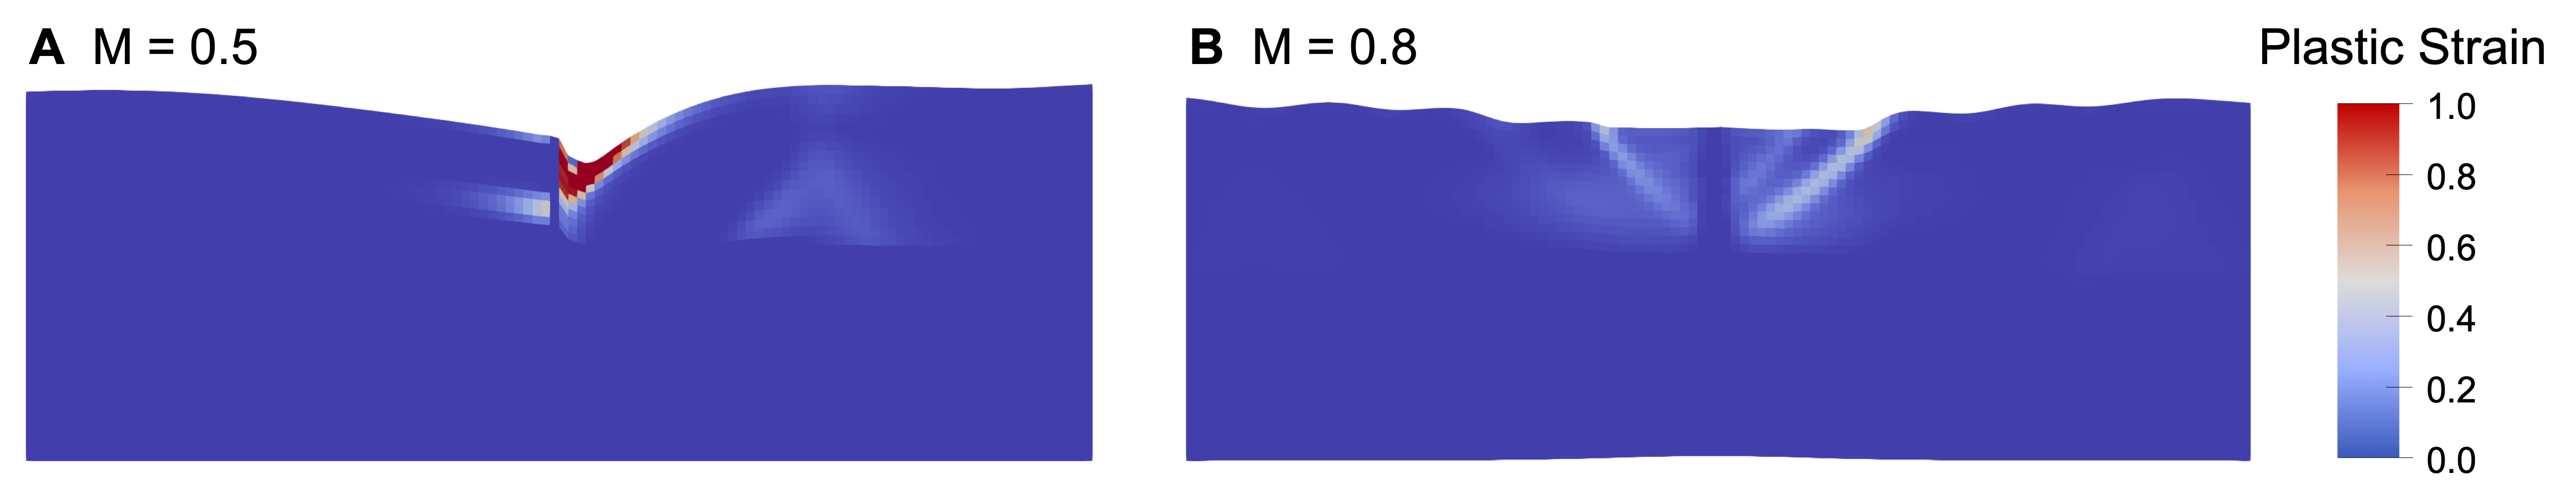
\includegraphics[width=0.99\linewidth,trim=8 8 8 8,clip]{./figs/f0fault.png}
	\caption{\textbf{A.} Snapshots of fault behavior of the $(\boldsymbol{F_{res}})_x=0$ model for M = 0.5 after 1Myr. Model shows detachment faulting. \textbf{B.} Same as \textbf{A} but for M = 0.8. Model shows alternating faulting.}
	\label{fig:f0fault}
\end{figure}

Filtered mean plate velocities are overall constant in time. $\overline{\boldsymbol{v}_x}$ is supposed to be constant because net forces on the side boundary nodes are zero and therefore the time rate of change of velocity should be zero on those nodes. For M = 0.5, $\overline{\boldsymbol{v}_x}$ of the plate moving to the left is 2.50 cm/yr and to the right is 2.50 cm/yr (Figure \ref{fig:f0mhv}A) with error of 0.5 cm/yr. When M = 0.8, $\overline{\boldsymbol{v}}_{x}$ remain constant at 2.70 cm/yr on the left-moving plate and 2.80 cm/yr on the right plate until the model ends (Figure \ref{fig:f0mhv}B).

%Mean plate velocities are overall constant in time but show minor temporal variability. $\overline{\boldsymbol{v}_x}$ is supposed to be constant because net forces on the side boundary nodes are zero and therefore the time rate of change of velocity should be zero on those nodes. However, while variability is not large compared to 2.5 cm/yr, the intended magnitude of $\overline{\boldsymbol{v}_x}$, $\overline{\boldsymbol{v}_x}$ is not exacly 2.5 cm/yr and changes over time slightly. \note[EC]{Leave only the description of the filtered velocity.} For M = 0.5, $\overline{\boldsymbol{v}_x}$ of the plate moving to the left is $-$2.50 cm/yr (Figure \ref{fig:f0mhv}A). $\overline{\boldsymbol{v}}_{x}$ of the plate moving to the right stays near this magnitude but seems to slightly increase from 2.50 cm/yr to 2.70 cm/yr by the end of the simulation. Filtered velocity do not exhibit this variability. When M = 0.8, $\overline{\boldsymbol{v}}_{x}$ remain constant at 2.70 cm/yr on the left-moving plate and 2.80 cm/yr on the right plate until the model ends (Figure \ref{fig:kmhv}B).
%From 400 to 520 Kyrs and 780 to 900 Kyrs, $\overline{\boldsymbol{v}_x}$ of both left-and right-side reduce (Figure \ref{fig:f0m08}).
%$\overline{\boldsymbol{v}_x}$ has two phases (Figure \ref{fig:f0mhv}B). From 200 to 400 Kyrs, the right-side plate is in a high-velocity phase and the left-side plate is in a low-velocity phase. From 400 to 600 Kyrs, now the right-side plate is in a low-velocity phase and the left-side plate is in a high-velocity phase. This pattern repeats until the model ends.
%
\begin{figure}[!htb]
	\centering
	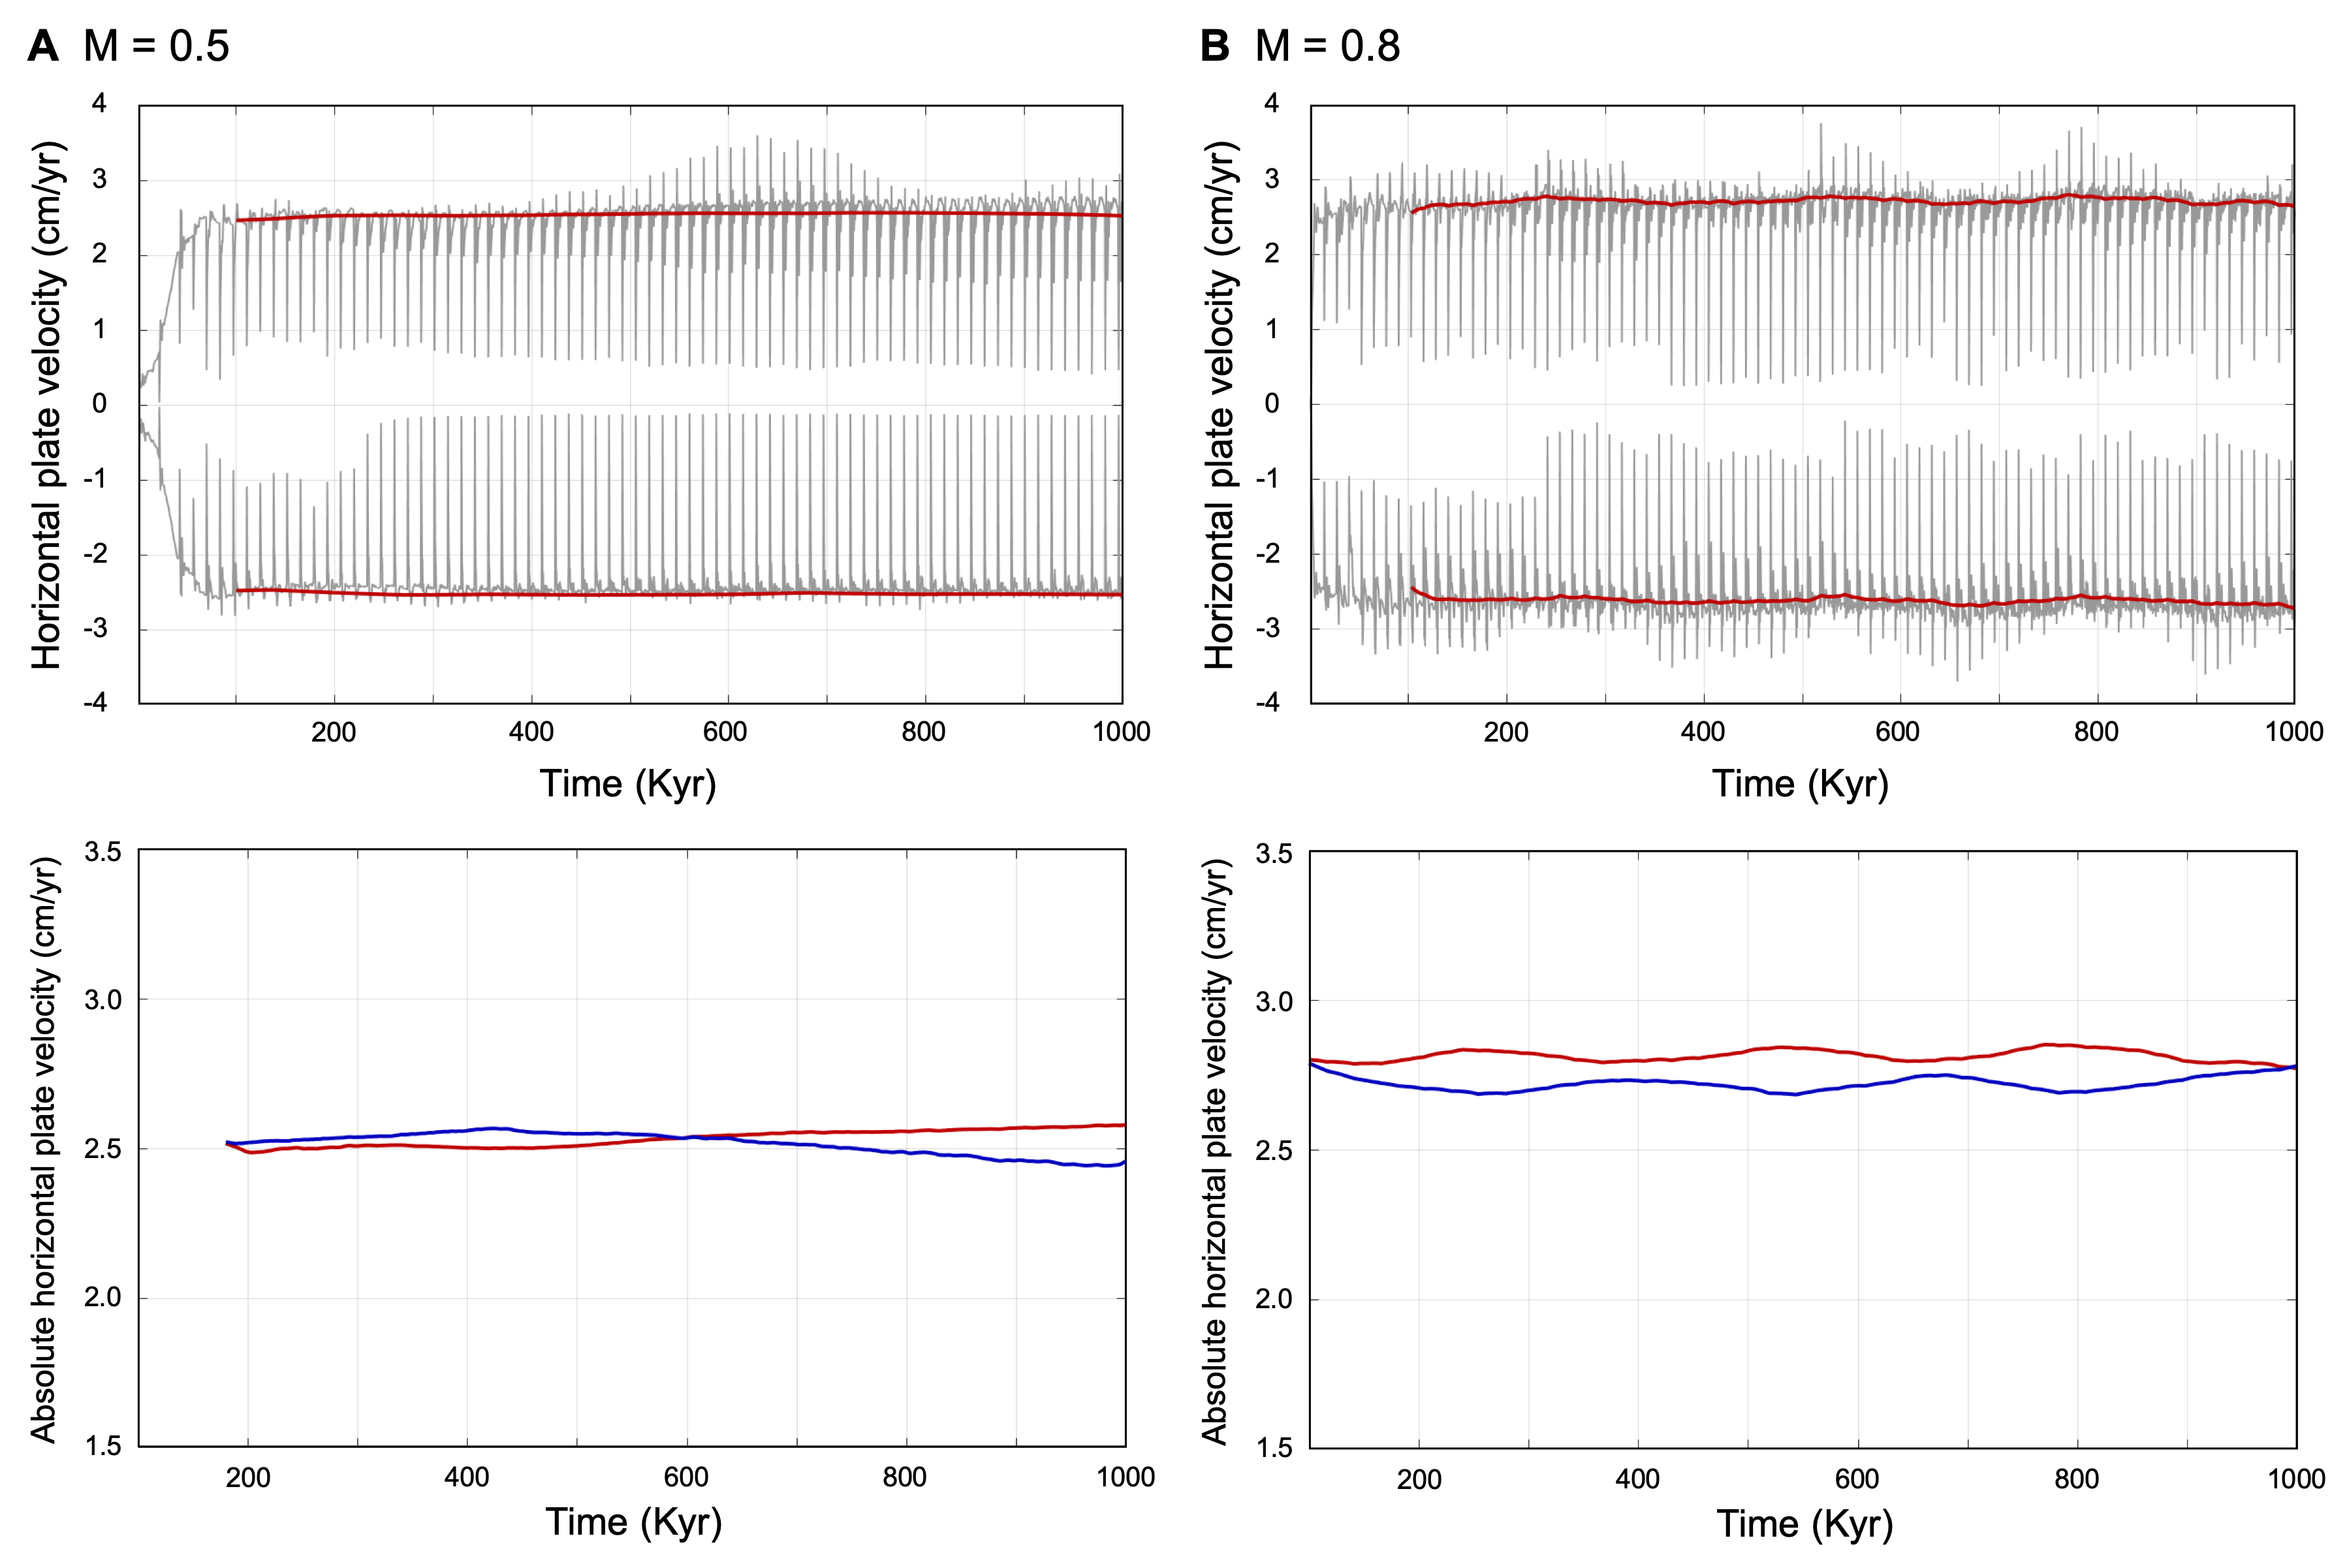
\includegraphics[width=0.98\linewidth,trim=4 4 4 4,clip]{./figs/f0mhv.png}
	\caption{\textbf{A.} (Up) Mean horizontal plate velocity obtained from M=0.5 $(\boldsymbol{F_{res}})_x=0$ model results. Red lines are filtered velocity. The positive values represent the right-moving plate and the negative values represent the left-moving plate. (Down) Absolute value of filtered velocity. Blue line is left-moving plate and red line is right-moving plate. \textbf{B.} Same as \textbf{A} but for M = 0.8.}
	\label{fig:f0mhv}
\end{figure}

\section{Constant $(\boldsymbol{F_{bdy}})_x$ models}

A constant $(\boldsymbol{F_{bdy}})_x$ implies that $(\boldsymbol{F_{res}})_x$ changes over time as $(\boldsymbol{F_{int}})_x$ evolves. Since the net residual force keeps changing, plate velocity under this condition is also expected to change in time.

Faulting styles are again consistent with the known correspondence to a given value of M. %Modeled fault behaviors from constant $(\boldsymbol{F_{bdy}})_x$ models are similar to that of kinematic models and  $(\boldsymbol{F_{res}})_x = 0$ models. 
For M = 0.5, a master detachment fault forms on one side (Figure \ref{fig:fbfault}A). For M = 0.8, the model produces a series of small-offset faults on both sides from the ridge axis (Figure \ref{fig:fbfault}B).
%
\begin{figure}[!htb]
	\centering
	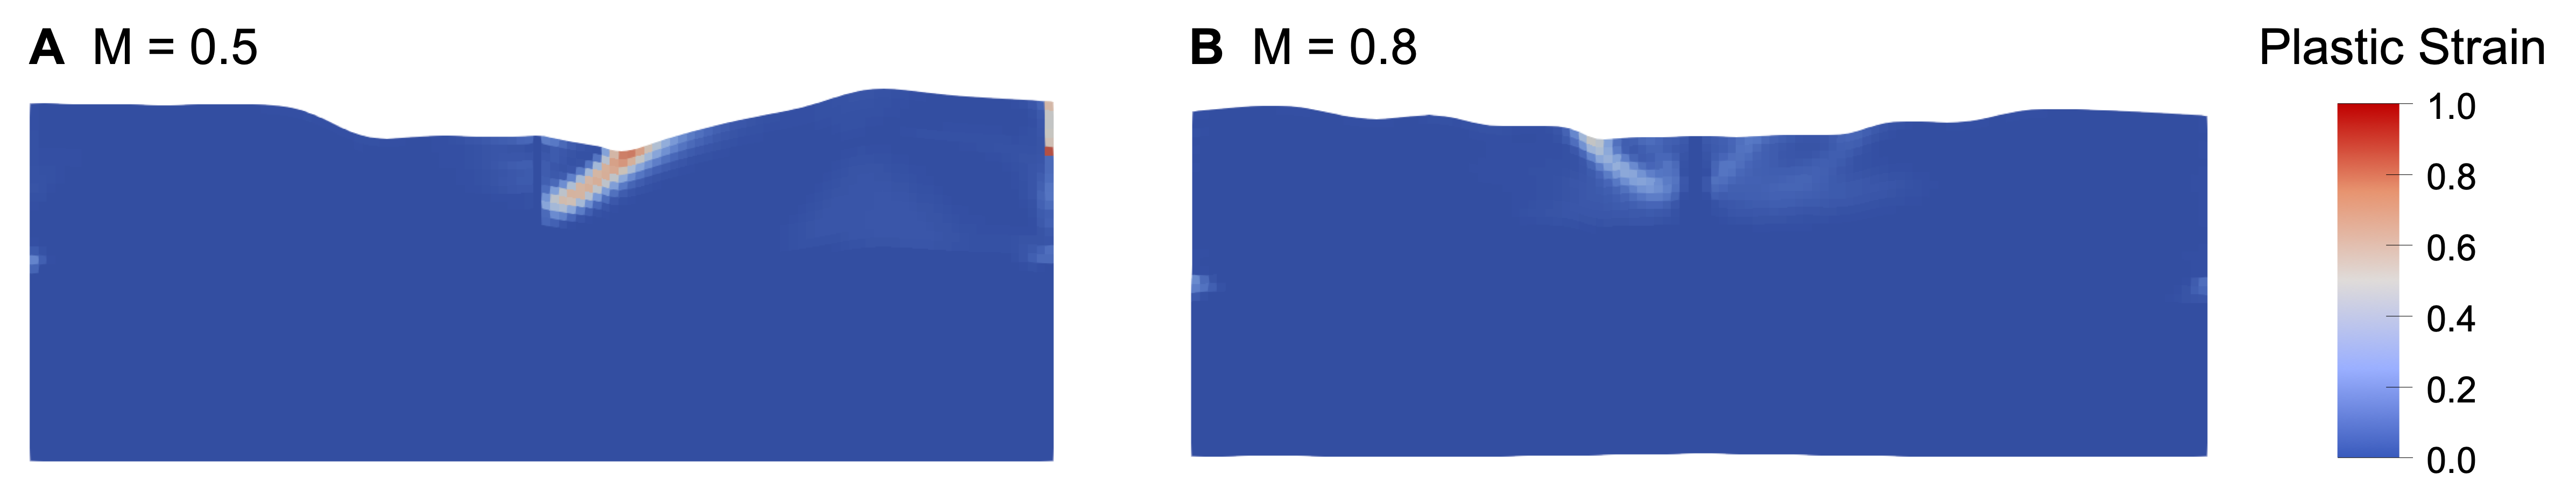
\includegraphics[width=0.99\linewidth,trim=8 8 8 8,clip]{./figs/fbfault.png}
	\caption{\textbf{A.} Snapshots of fault behavior of the constant $(\boldsymbol{F_{bdy}})_x$ model for M = 0.5 after 600 Kyrs. Model shows detachment faulting. \textbf{B.} Same as \textbf{A} but for M = 0.8 after 1 Myr. Model shows alternating faulting.}
	\label{fig:fbfault}
\end{figure}

Models in this group show significant temporal variations in $\overline{\boldsymbol{v}_x}$. 
% changes over time, although the amplitudes of abnormal peaks are great. 
When M = 0.5, the left-side plate $\overline{\boldsymbol{v}_x}$ keep changing in the range between 1 cm/yr and 2 cm/yr. The right-side plate velocity initially increase up to 2.4 cm/yr, and decrease to less than 1.0 cm/yr until the model ends (Figure \ref{fig:fbmhv}A).
When M = 0.8, plate velocities change more vigorously than other models (Figure \ref{fig:fbmhv}B). Until 250 Kyrs, the left-side plate $\overline{\boldsymbol{v}_x}$ decrease by 2.2 cm/yr, while the right-side plate  $\overline{\boldsymbol{v}_x}$ increase from 2.0 cm/yr to 2.7 cm/yr. From 250 to 380 Kyrs, left-side plate moves in constant rate and right-side plate moves rapidly. From 380 to 520 Kyrs, now the left-side plate moves rapidly and the right-side plate moves slowly. From 520 to 700 Kyrs, the left-side plate $\overline{\boldsymbol{v}_x}$ decrease to 2.1 cm/yr and the right-side plate $\overline{\boldsymbol{v}_x}$ increase up to 2.6 cm/yr. From 700 to 780 Kyrs, the left-side plate moves rapidly and right-side plate moves at a constant rate. After 780 Kyrs, the right-side plate moves rapidly until the model ends, while the left-side plate moves rapidly until 880 Kyrs, then moves slowly afterwards.
%Unlike velocity-driven model, force-driven model shows significant velocity changes over time. The detachment fault forms at 50Kyrs on left side of the spreading axis. After *yrs, the left plate moves slowly.
%
\begin{figure}[!htb]
	\centering
	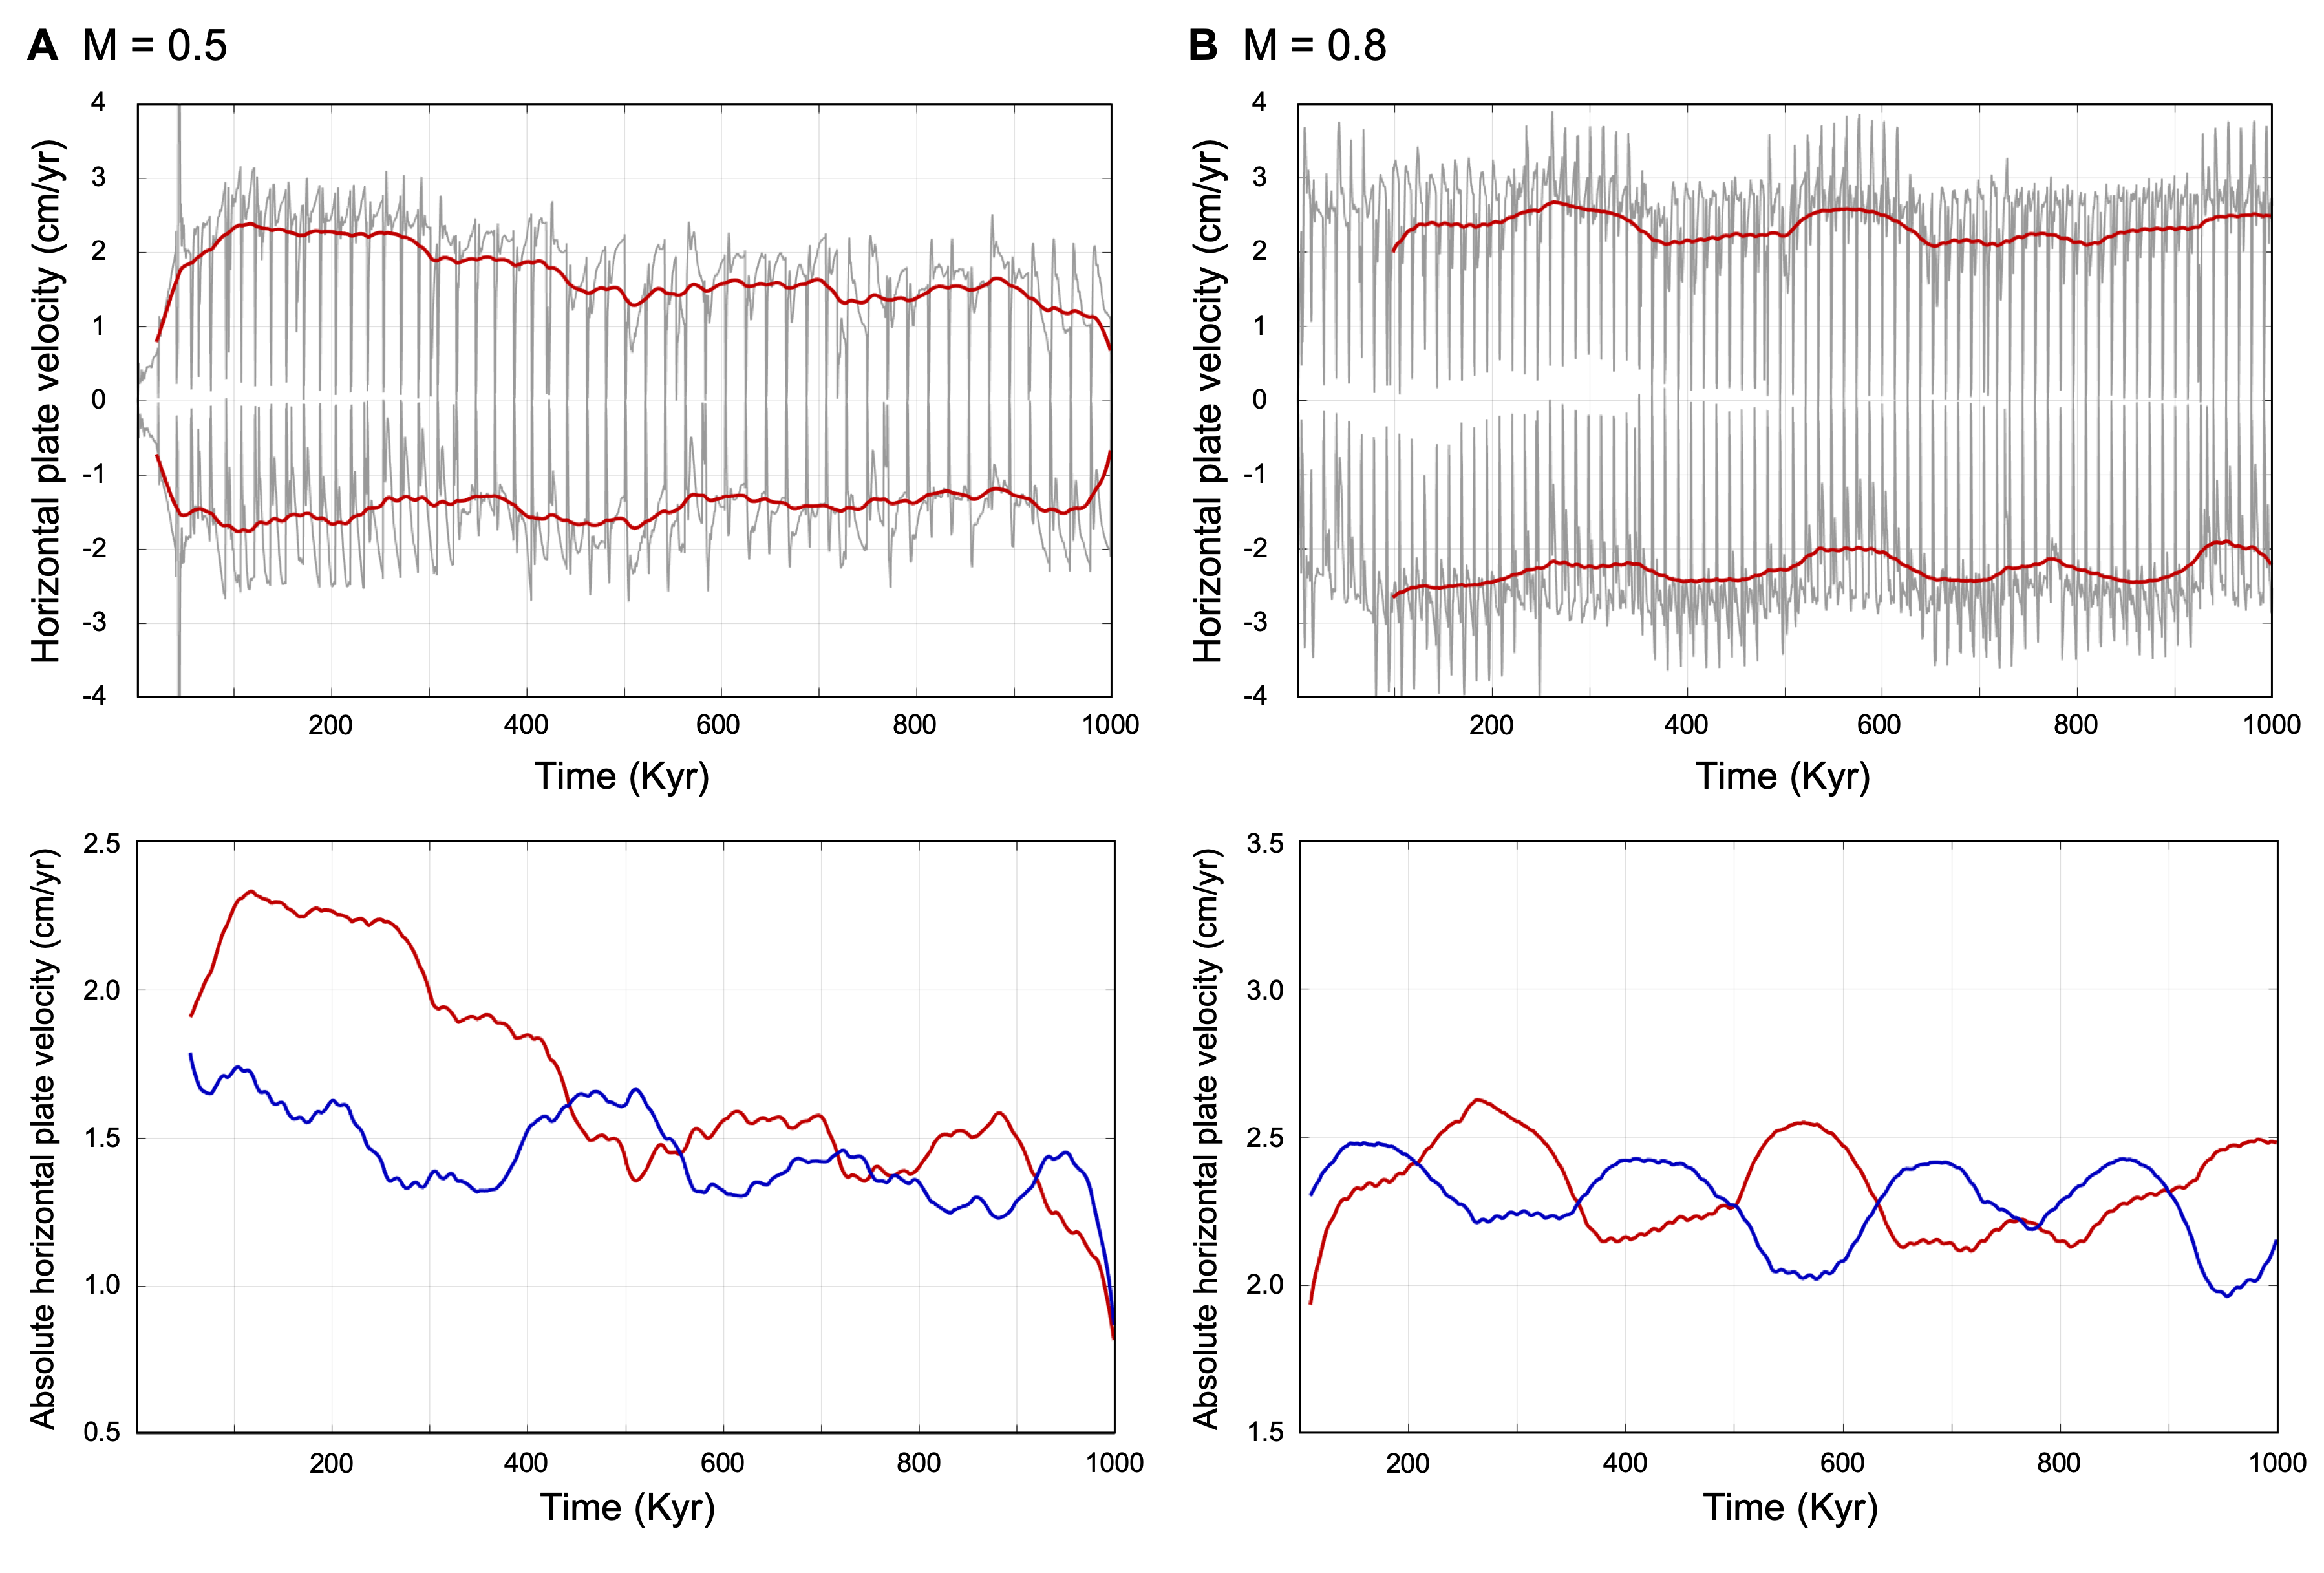
\includegraphics[width=0.98\linewidth,trim=4 4 4 4,clip]{./figs/fbmhv.png}
	\caption{\textbf{A.} (Up) Mean horizontal plate velocity obtained from M=0.5 constant$(\boldsymbol{F_{bdy}})_x$ model results. Red lines are filtered velocity. The positive values represent the right-moving plate and the negative values represent the left-moving plate. (Down) Absolute value of filtered velocity. Blue line is left-moving plate and red line is right-moving plate. \textbf{B.} Same as \textbf{A} but for M = 0.8.}
	\label{fig:fbmhv}
\end{figure}

\chapter{Discussion}

%Mean horizontal velocity of plates in the models includes the fault development at a ridge. Not to consider this faulting effects, I used $\overline{\boldsymbol{v}}_{x}$, $x$ component of the nodal velocities averaged over the nodes on each side of $\sim$15 km from the ridge axis. As a result, kinematic models show constant value of $\overline{\boldsymbol{v}}_{x}$ regardless of M factors.

%In kinematic models, normal faults migrate away from the axis at a rate $2v_p($M$-0.5)$, where $v_p$ is a constant plate-driving velocity (Figure \ref{fig:hangingwall}) \citep{Buck2005}. The plate containing an active fault is slower than the other plate. When M = 0.5, A master detachment fault forms on one side and do not move and hence the plate velocities remain constant value, with one plate moves faster than another. When M = 0.8, faults initiate near the ridge axis and are rafted off-axis. The new fault is antithetic and forms on the opposite side of the ridge axis from the original fault. In this reason, the models have repeated two phase plate velocity corresponding to the alternating faulting mode. Not to consider this faulting effects, I used $\overline{\boldsymbol{v}}_{x}$, $x$ component of the nodal velocities averaged over the nodes on each side of $\sim$15 km from the ridge axis and it remains constant.
%
%\begin{figure}[!htb]
%	\centering
%	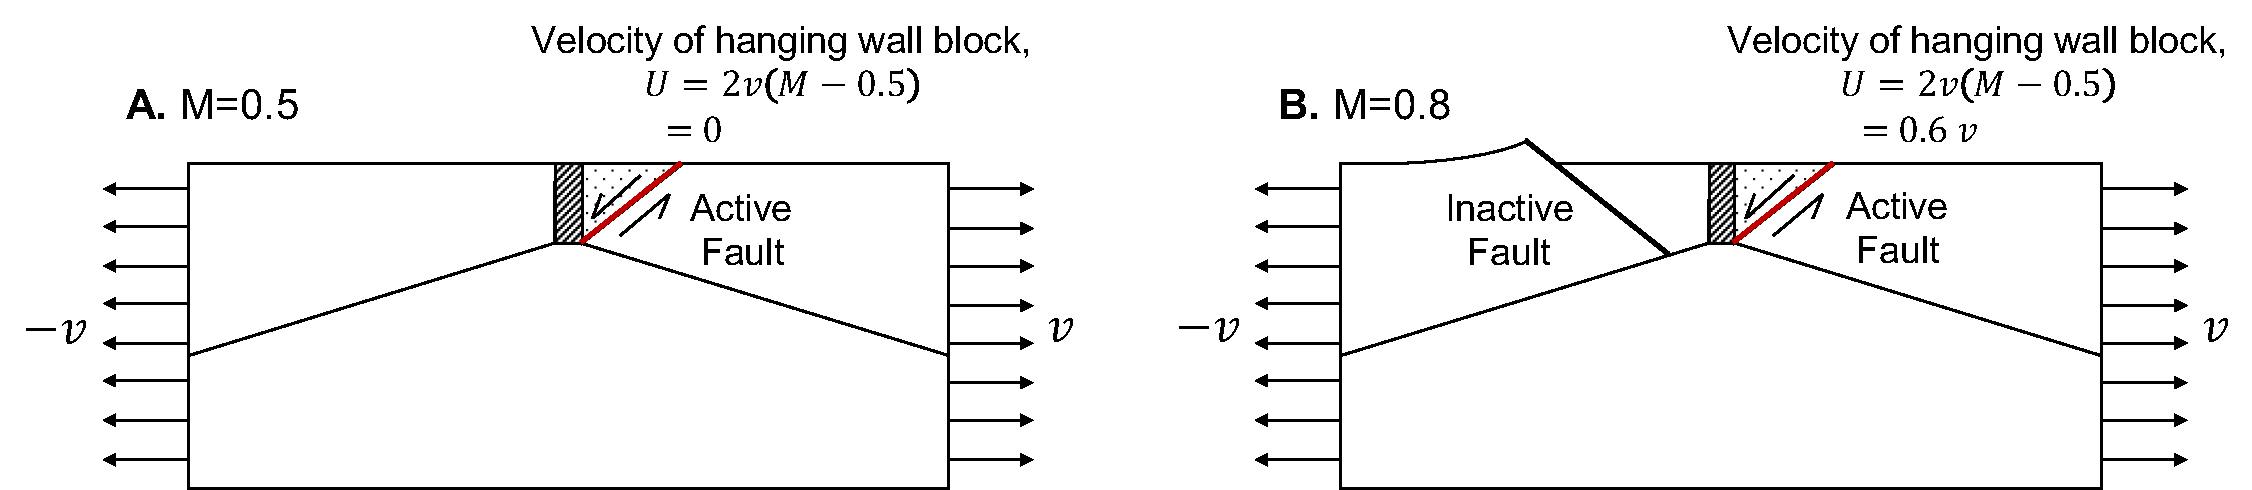
\includegraphics[width=0.99\linewidth]{./figs/hangingwall.pdf}
%	\caption{\textbf{A.} Schematic model showing velocity of a plate including active fault at mid-ocean ridges driven by velocity when M = 0.5. \textbf{B.} Same as \textbf{A} but for M = 0.8.}
%	\label{fig:hangingwall}
%\end{figure}

Changes of mean plate velocity over time in the Case II models appear connected to the evolution of the fault.
When M = 0.5, $\overline{\boldsymbol{v}}_{x}$ of the plate moving to the right seems to slightly increase from 2.50 cm/yr to 2.70 cm/yr by the end of the simulation, although the filtered velocity do not exhibit this variability. Connection of this change to the evolution of the detachment fault is suggested by the observation that the plate on the left does not develop a fault and its $\overline{\boldsymbol{v}}_{x}$ remains constant (Figure \ref{fig:f0mhv}A). When M = 0.8, from 200 to 350 Kyrs, the left-side plate moves slowly and right-side plate moves rapidly. From 350 to 510 Kyrs, now the left-side plate moves rapidly and right-side plate moves slowly. Although variability is about 0.1 cm/yr, $\overline{\boldsymbol{v}}_{x}$ show repeated two phase $\overline{\boldsymbol{v}}_{x}$ on both side, and it coincides with the alternating faulting. 

%$\overline{\boldsymbol{v}}_{x}$ remains at 2.7 and 2.8 cm/yr for the left and right plates, respectively. 
%\annote[EC]{the models show repeated two phase $\overline{\boldsymbol{v}}_{x}$ on both side of plates, and it coincides with the alternating faulting. }{This sentence used to be commented out but if true, restore it. Do you think the new thesis sentence of this paragraph can be supported by both M=0.5 and M=0.8 models? If not, what should be the summary statement of the variable mean plate velocity?}
%
%Even after averaging over the nodes on each side of $\sim$15 km from the ridge axis, $(\boldsymbol{F_{res}})_x=0$ models show small changes in $\overline{\boldsymbol{v}}_x$ corresponding to the faulting. Comparing to the kinematic models, the plate speed of the models with $(\boldsymbol{F_{res}})_x=0$ condition more strongly affected by faulting style.

Mean plate velocities show the greatest temporal variations in the Case III models where balance between $(\boldsymbol{F_{int}})_x$ and applied $(\boldsymbol{F_{bdy}})_x$ drives the plate motions. The magnitude of $\overline{\boldsymbol{v}}_{x}$ variations is greater in this group of models than in the Case I and II models. When M = 0.5, $\overline{\boldsymbol{v}}_{x}$ has an initial magnitude of $\sim$2.5 cm/yr but keeps changing until the model ends although perturbations from remeshing obscures the plate velocity. When M = 0.8, $\overline{\boldsymbol{v}}_{x}$ semi-periodically changes between 2 to 3.5 cm/yr until the model ends. However, noise from remeshing is strong in this model, too. 

%Overall, $\overline{\boldsymbol{v}}_{x}$ apparently change in force-driven models, while kinematic models only show constant values. With both M = 0.5 and 0.8, $\overline{\boldsymbol{v}}_{x}$ change more than 1 cm/yr over 1 Myr. However, it is hard to conclude that $\overline{\boldsymbol{v}}_{x}$ are in meaning range of plate velocity change
%clearly come from force boundary conditions
%, because remeshing effects could not be perfectly removed. The amount of changes in $\overline{\boldsymbol{v}}_{x}$ is in the range of changes of remeshing noise. The more the models are complex, the less the models are stable and hence generate more noise from remeshing.

Two ways of reducing numerical noise due to remeshing have been tested: Remeshing frequency adjustment and time step size adjustment.
Extracting mean plate velocities from numerical models is essential for investigating the fundamental question, whether the balance between plate-driving and resistant forces can explain time-variable plate growth. However, remeshing-induced noise is so strong that analysing the model results suffers ambiguity as discussed above. As a potential solution, remeshing frequencies in force-driven models were manually adjusted to reduce remeshing noise. This treatment is based on the observation that amplitudes of remeshing noise %produced from remeshing process 
are proportional to remeshing intervals. In other words, the less frequently remeshing occurs, the greater the noise amplitudes are. I tried 1 Kyr$^{-1}$ to 10 Kyr$^{-1}$ as forced remeshing frequencies. Increasing remeshing frequency helped diminishing the noise. However, models with frequent remeshing often failed to reproduce expected faulting style. Another treatment tested is to adjust time step size such that it is reduced immediately after the remeshing and increased linearly to its original value over the next 1000 time steps. This way, the remeshing effects are damped out while progressing only little in model time. In Case a shown in Figure \ref{fig:dtadj} as a red line, time step size ($\text{d}t$) is decreased to 10\% of the original value right after a remeshing event. In Case b (green in Figure \ref{fig:dtadj}), $\text{d}t$ is decrease only to 80\% of the original value. In Case c (blue in Figure \ref{fig:dtadj}), $\text{d}t$ is decreased to 10\% of the original value but increased back over the next 2000 time steps. Compared to the original $\overline{\boldsymbol{v}}_{x}$ plot (Figure \ref{fig:remeshing}A), none of these $\text{d}t$ adjustments lead to significant reduction of noise (Figure \ref{fig:remeshing}B and C). %This results suggest that adjusting size of time step does not remarkably affect the remeshing noise. 
The most effective treatment is to let the reduced $\text{d}t$ recover over the next 2000 time steps and exclude the first 1000 steps after each remeshing event from the mean plate velocity calculation. As shown in Figure \ref{fig:remeshing}D, this method shows notable improvement in diminishing the remeshing-induced perturbations in mean plate velocities. However, a more thorough study is still needed because this treatment sometimes cause faults to form in near-boundary or off-axis regions in Case III models.
%
\begin{figure}[!htb]
	\centering
	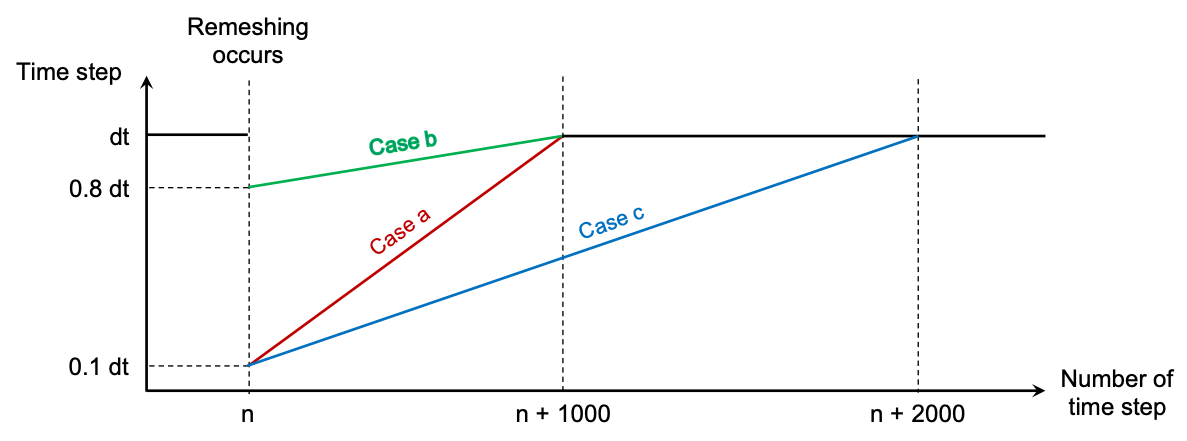
\includegraphics[width=0.8\linewidth]{./figs/dtadjust.png}
	\caption{Conceptual sketch showing adjusting time step method. Red line is Case a, decreasing time step to 10\% of original value. Green line is Case b, decreasing time step to 80\% of original value. In both Case a and b, the size of time step recover over the next 1000 time steps. In Case c, the size of tome step recover over the next 2000 time steps.}
	\label{fig:dtadj}
\end{figure}
%
% to dampen the remeshing effects will be needed to explore how the plate velocity change in the models. 
\begin{figure}[!htb]
	\centering
	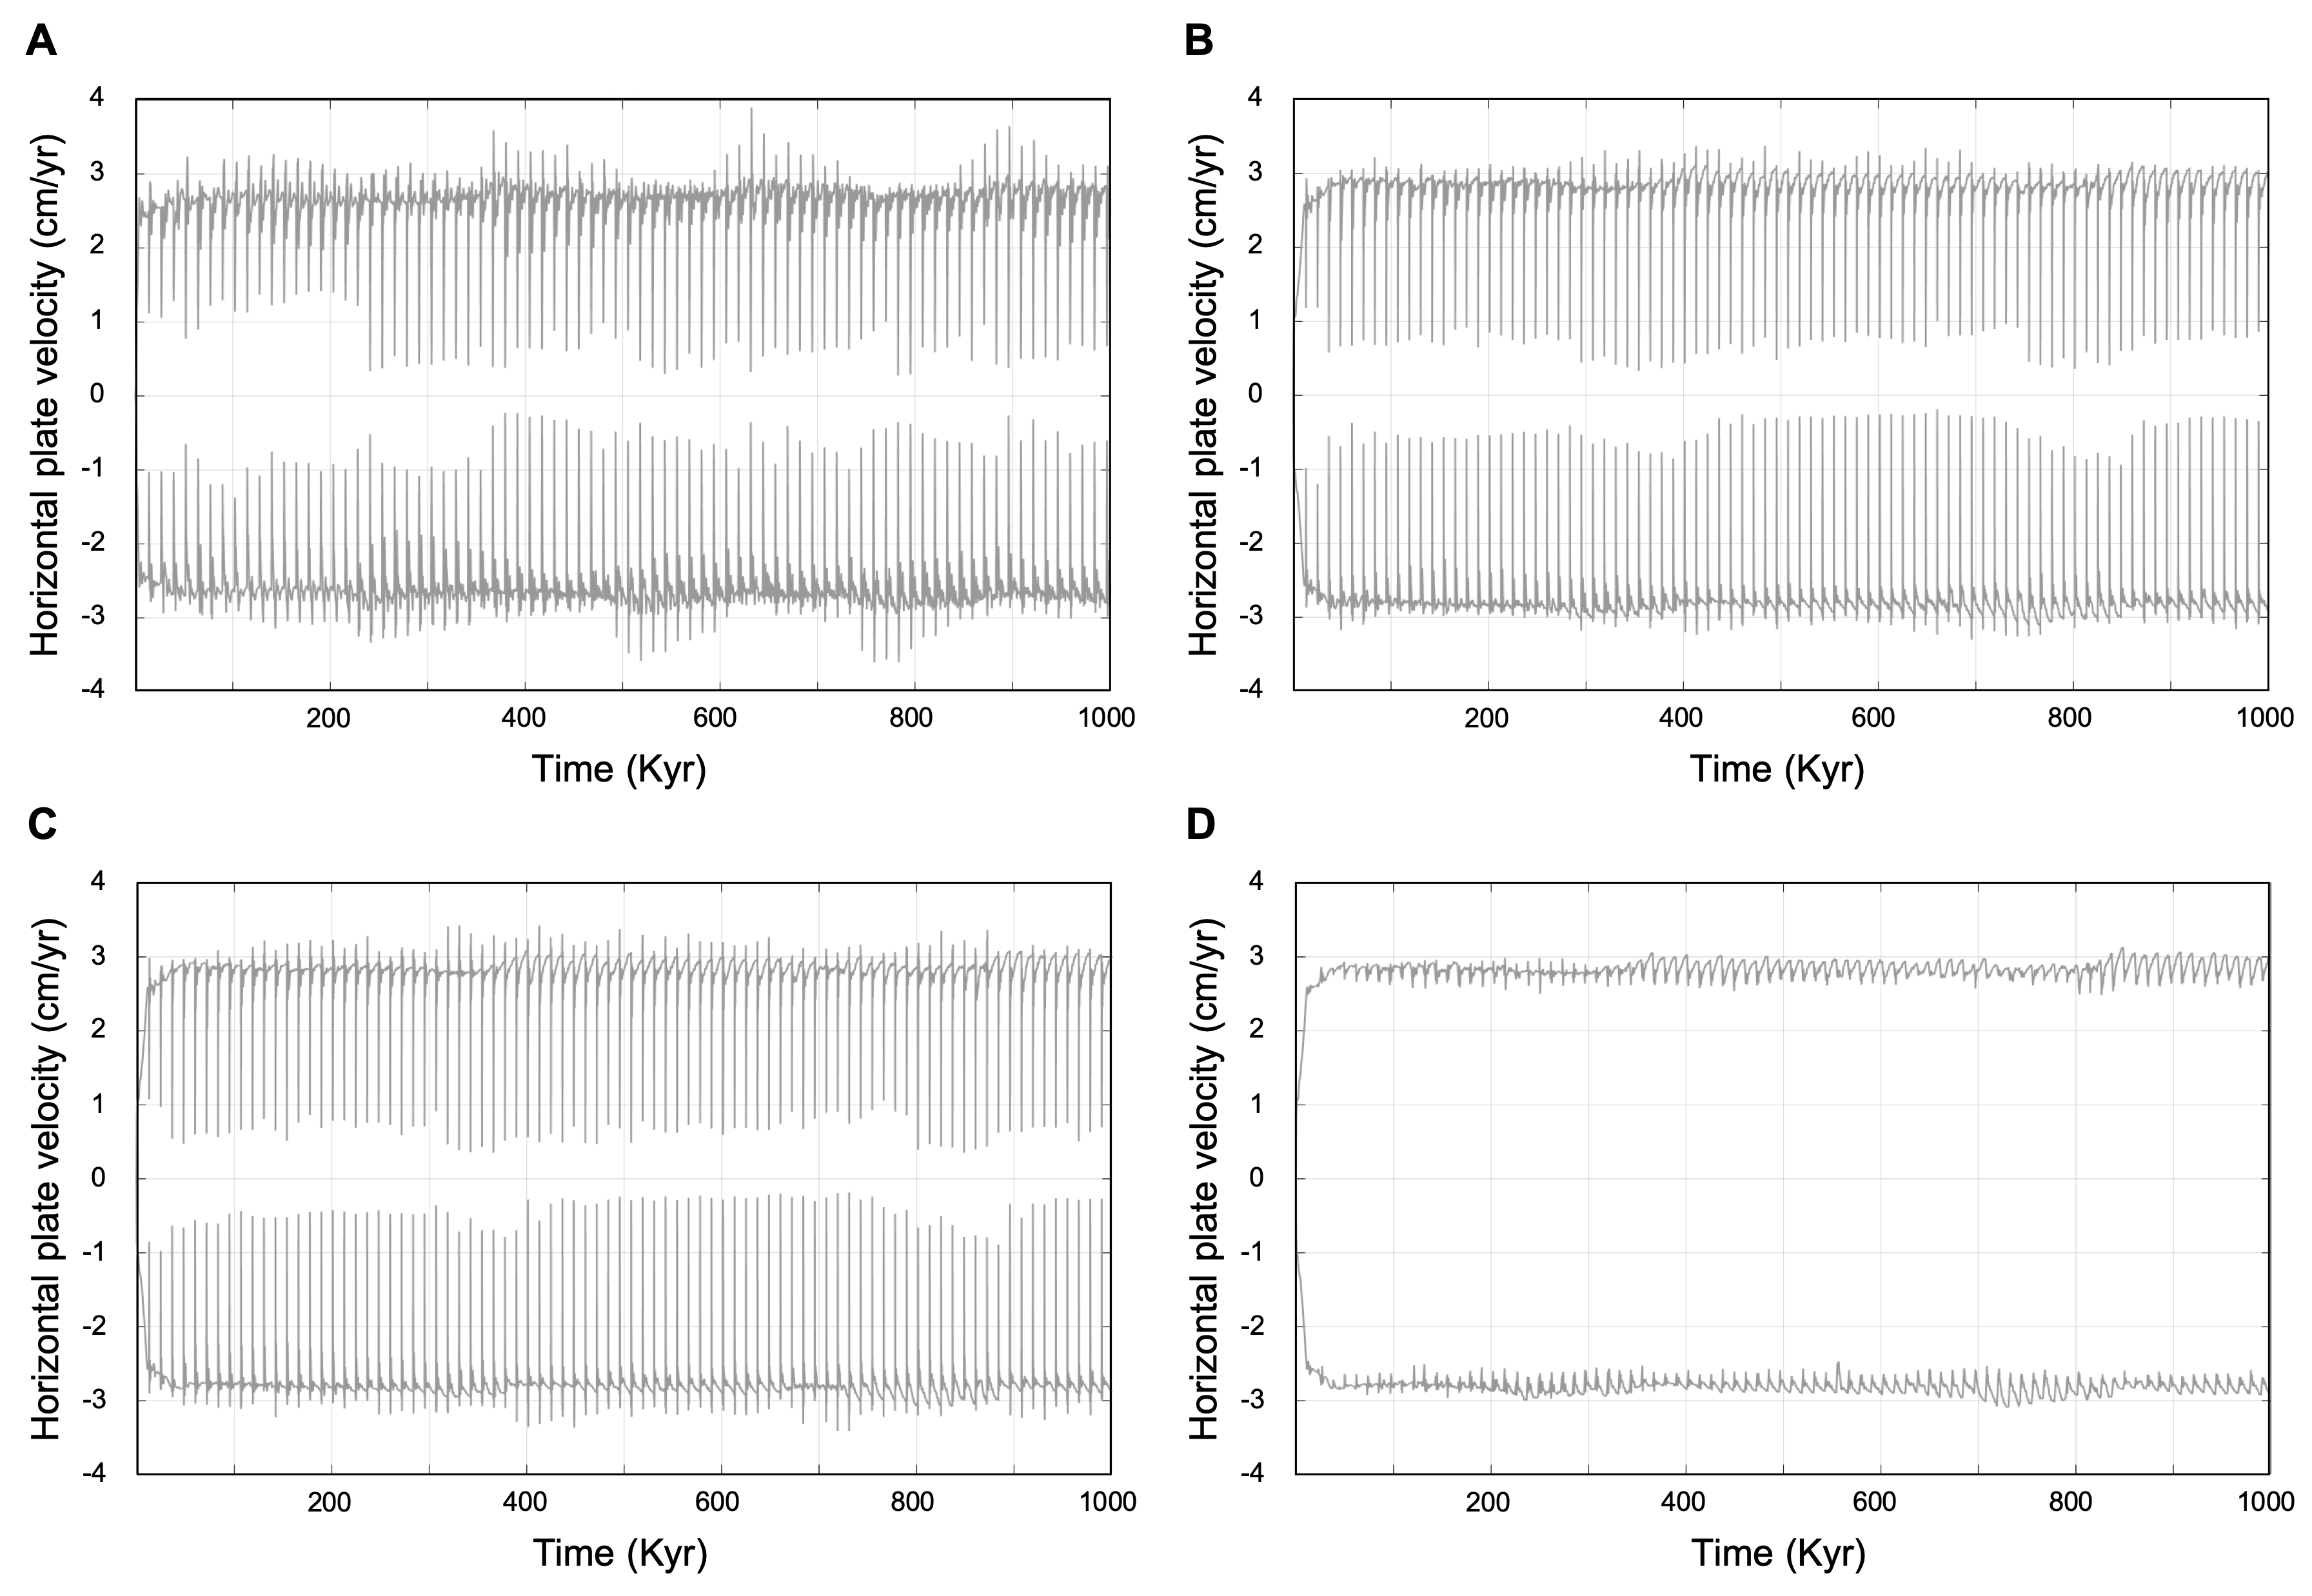
\includegraphics[width=0.98\linewidth,trim=4 4 4 4,clip]{./figs/remeshing.png}
	\caption{\textbf{A.} Raw mean horizontal plate velocity of M $=$ 0.8 $(\boldsymbol{F_{res}})_x = 0$ model. \textbf{B.} Mean horizontal plate velocity after case a filtering. \textbf{C.} Same as \textbf{B} but for case c. \textbf{D.} Mean horizontal plate velocity not printing the value over 200 time steps after remeshing events.}
	\label{fig:remeshing}
\end{figure}

In force-driven models like those of Case II and III, faulting styles might be sensitive to previously unrecognized parameter or components in the model setup rather than governed solely by the M factor. For instance, I observed that increasing $(\boldsymbol{F_{res}})_x$ slope affects the faulting mode. A slope of 1 Pa/yr leads to the detachment faulting, while slope of 10 Pa/yr or greater produce the alternating faulting mode for the same value of M. In general, a steeper slope for increasing $(\boldsymbol{F_{res}})_x$ favors the alternating faulting. Since the parameter M was invented based on conventional kinematic models, another parameter to represent magmatism in force driven mid-ocean ridge model might be necessary.

%To overcome aliasing issue, I printed $\overline{\boldsymbol{v}}_{x}$ values at every time steps. In this way, I verified that the abnormal peaks came from the remeshing events and obtained putative plate velocity. Still, the remeshing noise is not perfectly removed and confidence in $\overline{\boldsymbol{v}}_{x}$ is not sure.

%Similarly, in the cases of force-driven model, interaction between dynamic driving velocity from boundary force and opposite direction velocity from normal faults controls the plate speed in force. When half of total plate growth is accommodated by magma intrusion at spreading center, the velocity of one plate is always lower than another. Models produce repeated pattern of two-phase plate velocity when most of total plate spreading is taken up by dike.

%Besides these velocity variations, another affecting factor is observed in force-driven models, especially when M = 0.8. From 400 to 520 Kyrs and 780 to 900 Kyrs in $(\boldsymbol{F_{res}})_x=0$ model with M = 0.8, Both sides of $\overline{\boldsymbol{v}_x}$ reduce. In this time period, only the nodal velocities near dike zone and at the boundary are about 2.5 cm/yr, while inner plate nodal velocities are equal or less than 1 cm/yr. It may due to the internal force ($\boldsymbol{F}_{int}$) of the model. Resistance force occurring against the stretching force lag the plate to be grown.
%Besides these velocity variations, another fluctuation with greater amplitude and frequency is observed in constant $(\boldsymbol{F_{bdy}})_x$ models. Fault evolution is not sufficient to explain this long term and large magnitude variation. This fluctuation may come from the deep interior, as the feedback between deep mantle dynamics and surface plate motion. Hotter mantle conditioned models 

\chapter{Conclusions}

A new class of force-driven mid-ocean ridge numerical models are explored. 
%and oceanic lithosphereAs potentially new modeling approach to observed non-uniform plate growth, I tested three different boundary conditions in mid-ocean ridge models. All three cases show 
Based on the existing modeling techniques for simulating magmatism at the ridge axis and fautling, the models driven by force boundary conditions reproduce faulting styles corresponding to varying degrees of magmatism at the spreading center. They also exhibit significant differences in terms of mean plate velocities, suggesting great potential for further studies on non-uniform plate growth. In the models with prescribed boundary velocities, mean plate velocities remain constant. Varying the magmatism at the spreading center does not affect the plate speed. Thus, the observed variable rates of plate growth at mid-ocean ridge cannot be explained by existing kinematic models. When the residual forces, the sum of internal and boundary forces, vanish on the side boundaries, mean plate velocities are nearly constant as expected but also show time variability of a magnitude less than 0.2 cm/yr. The correspondence between the faulting styles and the degree of axial magmatism is still reproduced. The unexpected temporal variation in mean plate speed appears originating from the faulting since the small changes in plate speed is only observed in the plate containing a fault. %Therefore, $\overline{\boldsymbol{v}_{x}}$ is more strongly affected by faulting style than kinematic models. 
Models with a constant boundary force show greater variability in mean plate velocities, more than 1 cm/yr over 1 My, than in the kinematic models and those with zero residual boundary force. This magnitude of variability is greater than one third of original plate velocity regardless of faulting styles. These results suggest that force-driven model are a promising tool to investigate observed non-uniform plate growth. However, the employed numerical technique re-creates a mesh many times during a simulation and creates noise in the mean plate velocity records. Remeshing intervals and time step sizes were adjusted in a few different ways to reduce remeshing-induced noise. Although none of the tested treatments could successfully diminish remeshing noise without introducing other complications, some look promising and deserve further studies.

\bibliography{references}     % before changing bibliographystyle, remove *.bbl files in your working directory
\bibliographystyle{agsm.bst}  % the closest style to the University of Memphis Thesis Style Guide

\end{document}
